\chapter{The cross-platform compendium creation methodology and COMMAND 
system}\label{ch:command}
\chaptermark{Command}

\ldots

\instructionsintroduction


\todo(COMMAND: glossary ...)
GEO
ArrayExpress
SOFT
CEL
CDF
NCBI
EBI
MAGE-TAB
IDF
SDRF
ADF
MGED

\section{Introduction}

Microarrays are one of the main technologies for large-scale transcriptional
gene expression profiling.
%
To promot data sharing, scientific journals generally require the deposit of
these high-throughput experiments in public databases, such as Gene Expression
Omnibus (GEO) \cite{Barrett2011} or ArrayExpress \cite{Parkinson2009}, upon
publication.
%
These databases are an extremely rich source of information, containing freely
accessible data for thousands of experiments and a multitude of different
organisms, and in theory provide an opportunity to analyse gene expression of a
particular species at a global level.
%
They hold the potential to expand the scope of any smaller scale study: mining
the information contained in such databases offers molecular biologists the
possibility to view their own dedicated experiments and analysis in light of
what is already available.
%
So far however, this wealth of public information remains largely untapped
because these databases do not allow for a direct and integrated exploration of
their data.
%
The opportunity of combining all public experiments for a single organism has
not been explored due to practical issues that can ultimately be attributed to
the large heterogeneity inherent to microarray data.
%
Data sets originate from different experimenters or labs and microarrays do not
constitute a uniform technology.
%
Multiple microarray platforms exist and are manufactured in different ways.
Even for similar platforms, protocols for sample preparation, labelling,
hybridization and scanning can vary greatly.
%
Although community standards specifying the mandatory minimal experimental
information accompanying each dataset (e.g., MIAME \cite{Brazma2001}) have been
long established, the lack of the requirements \cite{Brazma2009} imposed
regarding the format of the platform descriptions and the expression
measurements, as well as the degree of preprocessing done on these values
further complicates the matter of experiment integration from a practical point
of view.


Despite such difficulties, several initiatives exist to actively build
expression compendia from public resources.
%
Most existing compendia can roughly be divided in two groups \cite{Fierro2008}:
those that directly integrate single-platform experiments, and those that
indirectly integrate cross-platform experiments.
%
Combining data from a single platform makes the in-between experiment
normalization and probe mapping relatively straightforward, so that the
quantitative measures of gene expression can be analysed directly across
experiments.
%
Most single-platform compendia databases, such as for instance
M$^{\textrm{3D}}$ \cite{Faith2008}, or the commercial Genevestigator
\cite{Hruz2008}, focus on Affymetrix, one of the more robust and reproducible
platforms \cite{Bammler2005, Irizarry2005}.
%
Combining data from different platforms, even to the extent of combining data
from single- and dual-channel microarrays, is generally done by indirect
meta-analysis as opposed to directly integrating the actual expression values:
one first applies the desired analysis procedure (e.g., identifying
differentially expressed genes, clustering gene expression profiles, etc.) on
each single data set within the compendium separately, and subsequently
combines the derived results.
%
These compendia are often topic-specific, collecting all publicly available
experimental information related to a subject matter of interest.  ITTACA
\cite{Elfilali2006} and ONCOMINE \cite{Rhodes2007}, for instance, focus on
cancer in human; Gene Aging Nexus \cite{Pan2007} on aging in several species.
%
There are exceptions though, such as the large ATLAS \cite{Kapushesky2010}
initiative from ArrayExpress.


The compendia created by directly integrating data across experiments have the
advantage of retaining actual expression values, which broadens the scope of
potential analysis procedures compared to indirect meta-analysis.
%
Most of such compendia center on eukaryotic organisms, for which considerable
amounts of data are available.
%
Relying on only one platform can still lead to sizeable compendia with a broad
scope in condition content, such as the human compendium constructed based on
the Affymetrix U133A platform with over 5000 samples \cite{Lukk2010}.  However,
for most species (e.g., \textit{Zea mays}), no single platform has such a
dominant role.
%
The worst is prokaryotes.  Even for model organisms such as {\it E. coli}, much
less data is available on individual platform and a significant portion of the
data is missed out when considering only one platform.


To have the advantage of the direct integration, while not being limited to a
single platform, we have devised methodology that directly combines expression
data across platforms and experiments.
%
The methodology has enabled us to create comprehensive compendia incorporating
most high quality public data covering a broad range of experimental conditions
as well as extensive types of biological samples.
%
To facilitate the creation of new compendium and the curation of the existing
ones, a software system COMMAND (Cross-platform cOMpendium MANagement Desktop)
is also developed, utilizing web browser as the front-end and our methodology
at the back-end.




\section{Methods}


%% \todo{COMMAND: reminder to be commented}
%% \textbf{REMINDER: Hurdles to create cross-platform exp compendium}

%% There are \textbf{three main hurdles} preventing direct data integration across
%% platforms and experiments.
%% %
%% \begin{itemize}
%% %
%% \item[exp-data] The lack of a consistent format to report expression data
%%   prevents an automatic and computerized data retrieve.
%% %
%%   The heterogeneity of microarray platforms hampers direct integration in two
%%   aspect.  The possible probe sequence differences of a gene across different
%%   platforms questions the compatibilities of the obtained measurements.
%% %
%% \item[metadata] The metadata describing biological sample and experimental
%%   conditions is provided as free text which is often incomplete and lack of
%%   consistency.  Standards like MIAMI \cite{Brazma2001, Brazma2009}, although
%%   promote human interpretation of experimental conditions, do not facilitate
%%   computational analysis.
%% %
%% \item[normalization] The different preprocessing algorithms employed by
%%   different experiments further complicates the data compatibility.
%% %
%%   The log ratio calculation, capable of removing certain technical variations
%%   from the normalized data, inherently improves the data consistency across
%%   platforms and experiments \cite{Shi2006, Shi2008}
%% %
%% \end{itemize}






\subsection{Cross-platform expression compendium}

Our expression compendium is essentially an organism-specific matrix of
expression values derived from publicly available microarray experiments which
are homogenized to make them comparable.
%
The rows of a compendium correspond to the known genes of the organism in
question constructed based on the corresponding RefSeq file at NCBI
\cite{Pruitt2007}.
%
Uniquely, each column of it is a `\textit{contrast}', which does not represent
single biological sample but the differences between a pair of samples, one as
test and the other reference.
%
Consequently, the expression values themselves are calculated as expression
log-ratios representing the gene expression changes induced by the differences
between this pair of samples.
%
Converting absolute measurements of expression into expression changes is the
principal means for rendering expression values comparable across platforms and
experiments.
%
Relative expression calculated intra-experiment/platform (i.e. between two
conditions measured in the same microarray experiment using one platform)
negates much of the platform and experiment specific variations that makes it
impossible to reliably compare the absolute quantities reported in different
experiments \cite{Shi2006}.



\subsubsection{The database schema for expression compendium}\label{sec:command-db-schema}
%% \todo{COMMAND: to be finished with a abstract schema in figure,
%%   Ref. MIAME2001, MIAMEPlant2006}

\begin{figure}
  \centering
  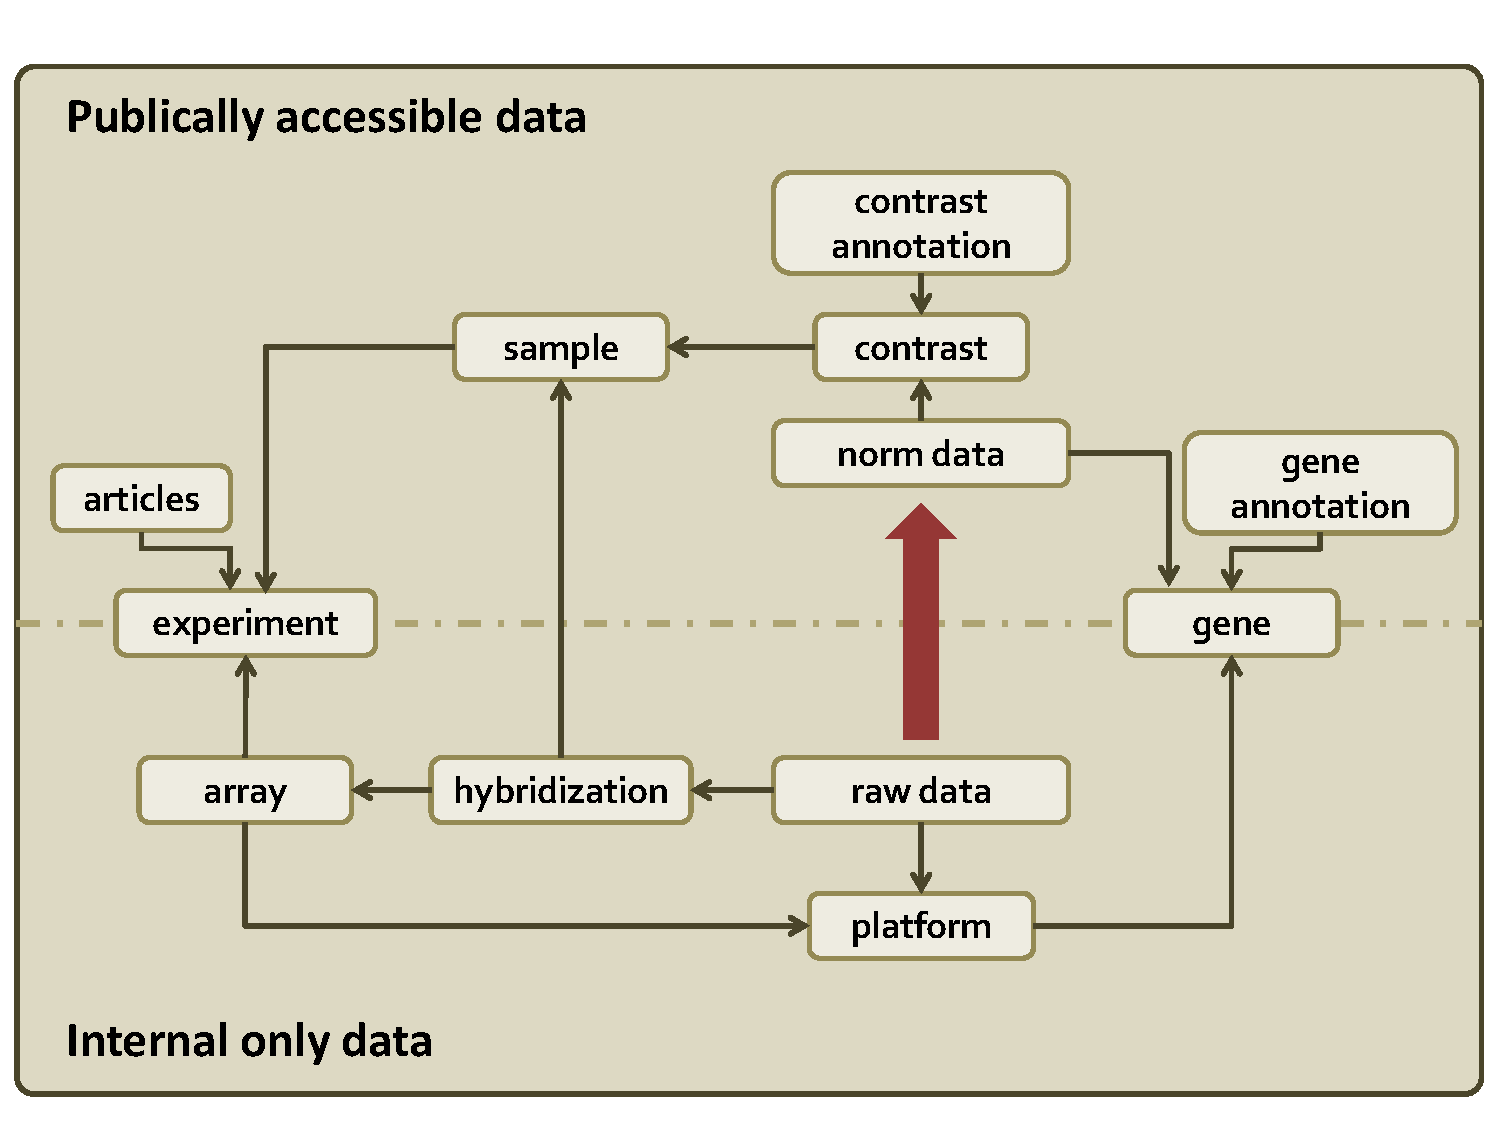
\includegraphics[width=1\textwidth]{DB_schema.pdf}
  \caption[The database schema for expression compendium]{ \textbf{The
      database schema for expression compendium}.
  }
  \label{fig:comp-db-schema}
\end{figure}

The compendium is stored in MySQL database. An abstract schematic
representation of various data content and their relation is shown in Figure
\ref{fig:comp-db-schema}.
%
The schema is separated into two parts. The entities in the upper part form
the data of a compendium, and are publicly accessible.
%
Those in the lower part are the data collected to build compendium, hence are
only accessible internally.

Here we briefly explain each entity in the schema.
%
A gene expression \textit{experiment} is composed of a set of related arrays
that are designed to obtain expression data in order to answer a biological
question.
%
An \textit{array} corresponds to one microarray in an experiment on which the
biological sample(s) are hybridized and the gene expression measurements are
generated.
%
A \textit{hybridization} refers to individual sample that is labeled and
hybridized on an array.
%
For an array using single-channel platform like Affymetrix, there is only one
hybridization per array.  Whereas there are two hybridizations, one per
channel, for the array using dual-channel platform.
%
A \textit{platform} denotes a specific microarray chip design and the
corresponding probe annotation information, such as, the probe sequence, the
physical layout, the target gene, etc.
%
The \textit{raw data} are original measurements of each probe grouped by
hybridization.  Three types of data are accepted, the raw expression value,
the background intensity, and the background corrected expression value.
%
A \textit{sample} refers to each individual biological sample that is used in
an experiment.  Biological duplicates are treated as different samples.
%
Note that a hybridization is an instance of a sample that is hybridized to a
specific microarray chip.  When the same biological sample are hybridized
onto several microarrays, they are referred as one sample but different
hybridizations in the compendium.
%
%% A \textit{contrast} as defined in previous section, specified a comparison
%% between a reference sample and a test sample.
%% %
%% The \textit{norm data} are log-ratios, each of which represents the expression
%% variation of one gene under one contrast in which the gene's expression level
%% in the test sample are compared with that of the reference sample.
%
As explained in previous section, a \textit{contrast} specifies a comparison
between a reference sample and a test sample, and the \textit{norm data} are
gene expression log-ratios.
%
We use a relaxed definition for \textit{gene}, which includes not only the
protein coding sequences, but also other sequences that are expressed and
functioning, given their expression level can be quantified.
%
There are also three supplementary entities, the article, the contrast
annotation, and the gene annotation.
%
The \textit{article} stores the publications related to an experiment.
%
The \textit{contrast annotation} contains, for each contrast, the sample
characteristics and the experimental factors that differ between the pair of
samples.
%
The \textit{gene annotation} stores the functional annotation of each gene
collected from external sources, including the metabolic pathway, Gene Ontology
annotation, transcriptional regulation, and the transcription unit.






\subsection{The compendion creation methodology}
\label{sec:colombos-comp-method}

\begin{figure}
  \centering
  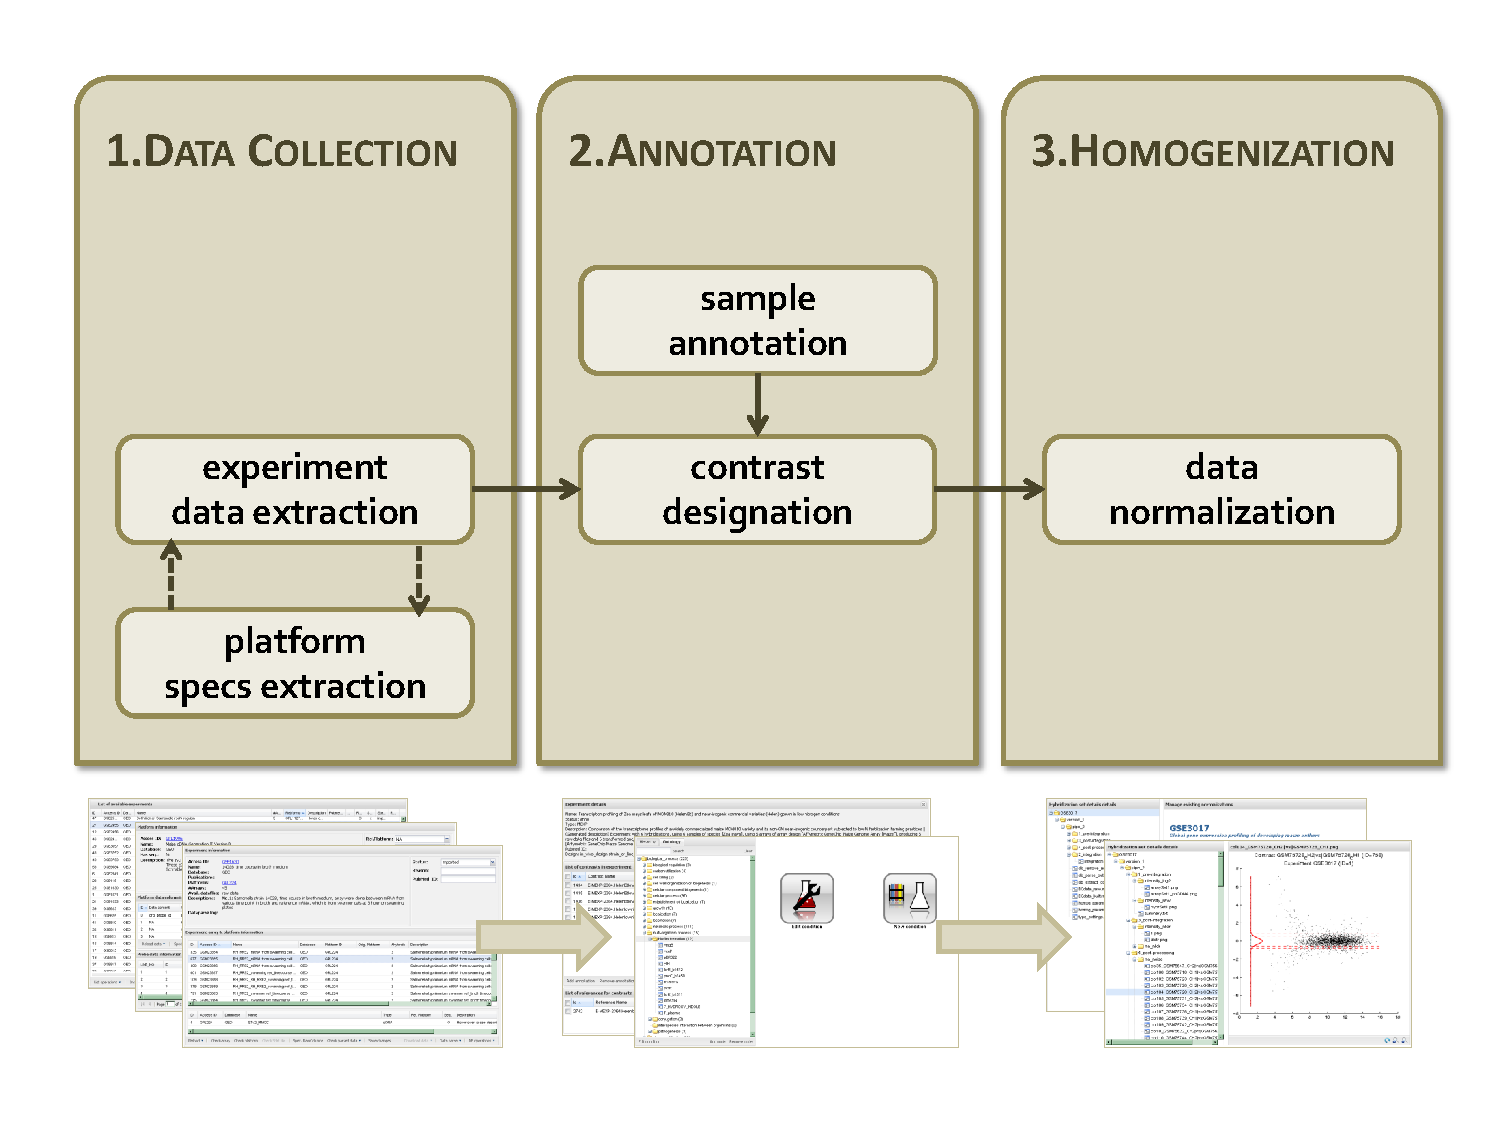
\includegraphics[width=1\textwidth]{COMMAND_Workflow.pdf}
  \caption[Cross-platform expression compendium creation methodology]{
    \textbf{Cross-platform expression compendium creation methodology}.  From
    left to right, three box represent three main steps of the cross-platform
    expression compendium creation methodology.  The corresponding
    functionalities are specified in the rectangles inside of each box.
    Below, the boxes shown the snapshots of the corresponding COMMAND
    interfaces.}
  \label{fig:command-workflow}
\end{figure}


The cross-platform compendium creation methodology is composed of three major
steps (Figure \ref{fig:command-workflow}), namely, data collection, experiment
annotation, and data homogenization.
%
First, in data collection step, the expression data and the accompany
(experiment and platform) information are retrieved from the online
repositories, overcoming the issue of the prevalent data representation
discrepancies.
%
Next in annotation step, the contrasts are constructed by assigning a pair of
samples, one as reference and the other as test.  The experimental factor and
the characteristic differences between two samples are curated manually for
each contrast and specified using a set of controlled in-house vocabularies.
%
At last, in data homogenization step, the raw expression data are normalized
and log-ratios are calculated based on the sample contrast designation to
create the compendium data matrix.
%
In the following sections, we will explain the individual step in detail.






\subsubsection{Data collection}

%% [Colomobos (v1) paper]
%%
%% The first step is the retrieval of microarray experiments and associated
%% platforms from Gene Expression Omnibus (GEO) and ArrayExpress. Representation
%% discrepancies prevalent in experimental data directly obtained from online
%% databases are systematically removed and the resulting data are then stored as
%% available in a uniform format. ‘As available’ does not necessarily equate to
%% raw scanner output, since there are no MIAME reporting standards regarding the
%% measurement units of expression \cite{Brazma2001, Brazma2009}. Often raw
%% intensities are not provided in the public databases (especially for older
%% experiments), and only already processed data are reported.

%% General issues to be covered
%% %
%% \begin{itemize}
%% \item free text for experimental information [metadata]
%% \item lack of standard format to report platform probe specification,
%%   sequence information is not always provided [probe specs]
%% \item raw data is not always required, if provided, lack of standard
%%   format to report raw data [raw data]
%% \item lack of platform type specification
%% \item the number of channels specification is provided in GEO Sample 
%%   record and can be derived from SDRF file from ArrayExpress [raw 
%%     data] 
%% \end{itemize}


%% Summary
To create compendium, the gene expression data need to be collected from
online public repositories, GEO and ArrayExpress.
%
Although community guidelines such as MIAME \cite{Brazma2001} exists, the
failure to provide a standard format to represent information of an expression
experiment causes widespread representation discrepancies among the data
deposited in those online repositories.
%
The prevailed discrepancies coupled with the colossal amount of the available
data makes the systematical expression data retrieval a daunting task.
%
To make this task viable, we develop a semi-automatic workflow designed to
tackle various data discrepancies and automate various processing procedures
to handle the huge volume of the data.

%Here, we first explain what data are available, then the different sets of data
%to be retrieved, at last, for each set of data, discuss the data issues related
%to its retrieval and our strategy to tackle them.  

Here, we first explain what data are available, then the different sets of data
to be retrieved, and at last, discuss the data retrieval issues and 
corresponding handling strategies for GEO and ArrayExpress separately, as each 
of them utilizes its own data reporting format and has its own specific data 
problems.



\paragraph{Data available at online repositories}\label{sec:command-data-content-online}

GEO and ArrayExpress, though both are MIAME-compilant, use different files and
formats to store information. % for an gene expression experiment.

%% http://www.ncbi.nlm.nih.gov/geo/info/overview.html
%% http://www.ncbi.nlm.nih.gov/geo/info/soft2.html
%
In GEO, there are two sets of data for an experiment, the \textit{GEO Series}
(GSE) containing the original submitted data and the \textit{GEO DataSet}
(GDS) containing curated normalized data.
%
To create compendium, we collect original data in GSE.
%
GSE data of an experiment is stored in a standard simple line-based plain text
format, called SOFT (Simple Omnibus Format in Text).  One SOFT file per GSE in
compressed (gzip) form.
%
The file contains one or multiple instances of three types of records: Series,
Sample, and Platform.
%
The \textit{Series} record contains general information about various
aspect of an experiment described in free text.  The references to the
corresponding Sample and Platform records are also provided.
%
The \textit{Sample} records corresponds to one microarray chip used in an
experiment.
%
It is composed of two sections.  The first one provides free text descriptions
about biological samples hybridized to the microarray, including information
about sample attributes and experimental factors crucial for compendium data
exploration and interpretation.
%
The reference to the related Platform record is also provided here.
%
In the second section, the gene expression measurements are reported for each
probe of the microarray in a tabular form. Often the values reported here are
processed data instead of the desirable original probe measurements.
%
The \textit{Platform} record describes the microarray chip used to measure
gene expression, including a free text description and its probe annotations
in a tab-delimited table.
%
Specific about the required content in various records and their sections, the
SOFT format does not impose strict requirements about the representation of the
data.
%
Consequently, the format used to report the expression values and the probe
annotations various among experiments and platforms.
%
Additionally, for many experiments, raw data files are available as
supplementaries providing an alternative source to obtain desirable gene
expression measurements.
%
However, as the submission of the raw data files is not mandatory, many
experiments do not have supplementaries.
%
In GEO, a unique access id is assigned to every record.
%
And the `Series', `Sample, and `Platform' record corresponds to the
experiment, array, and platform object respective in our compendium
(Fig. \ref{fig:comp-db-schema}).


%% www.ebi.ac.uk/miamexpress/help/index.html
%% www.ebi.ac.uk/miamexpress/help/datafile_help.html
%% 
%% www.ebi.ac.uk/fgpt/magetab/help/
%% 
%% www.ebi.ac.uk/training/online/course/arrayexpress-submitting-data-using-mage-tab
%% tab2mage.sourceforge.net/docs/magetab_docs.html
%%
%% www.ebi.ac.uk/arrayexpress/help/accession_codes.html
%
In ArrayExpress, the experiment data is stored in the MicroArray Gene
Expression Tabular (MAGE-TAB) format.
%
In this format, 4 types of file capturing different set of information are
used, namely, the Investigation Description Format (IDF) file, the Sample and
Data Relationship Format (SDRF) file, the Array Design Format (ADF) file, and
the raw and processed data files (normally packed into one zip file).
%
Similar to the `Series' record in GEO SOFT format, the \textit{IDF} file
provide an overview for an experiment.
%
Although the MGED ontology terms are used, they specify only the type of the
information.  The content, however, is still described in free text.
%
The \textit{SDRF} file describes the sample characteristics and the
relationship between samples, arrays, and data files.
%
The content is presented in a tabular form, in which each record (row)
describes information about one biological sample hybridized to a specific
channel of a specific microarray chip, hence corresponds to a hybridization in
our compendium (Fig. \ref{fig:comp-db-schema}).
%
The reference to the corresponding platform are provided for each record.
%
One caveat about the SDRF file is that its format is not strictly defined, and
can vary among experiments.
%
Next, the \textit{ADF} file provides information for a microarray platform,
including both the descriptive information and the probe annotations.
%
At last, the expression values are reported in the raw and/or normalized
data files.
%
In ArrayExpress, the unique access id is given only to experiment and
platform, which directly corresponds to the experiment and platform object
in our compendium (Fig. \ref{fig:comp-db-schema}).
%
However, there is no explicit record in ArrayExpress that corresponds to the
array object.  Additionally, although each record in SDRF file corresponds to
the hybridization object, without a unique reference, this information is only
indirectly accessible though the corresponding ArrayExpress experiment.
%
%% In ArrayExpress, the unique access id is given only to experiment and
%% platform. The sample or the hybridization information are only
%% indirectly accessible though the correponding experiment.

It should be noted that the raw data files reported in GEO and ArrayExpress
are in original vender specific formats, which differ among softwares.
%
Often allow to be used alone, in addition to the expression value(s), the
annotation are also provided for each probe in those files.







\paragraph{Data retrieval goal}\label{sec:command-data-goal}

There are three sets of information to be extracted, the experiment
metadata, the platform specification, and the raw expression values.
%
\todo{COMMAND: need to be explained in the introduction}
%
The experiment metadata describing the sample attributes and experimental
factors, which, as the drive of the observed gene expression changes, are
essential for the data exploration and interpretation.
%
Additionally, the metadata also specifies the relations between the samples
and the microarray platform used, and the corresponding data tables or files
containing the obtained values.
%
As the expression value is measured by individual probe of a microarray, the
measurements reported are for each probe instead of gene.
%
The platform specification contains the probe-to-gene correspondence that is
essential for converting probe measurements into gene expression values.
%
%% Additionally, the platform specification also provides clues about the
%% number of samples hybridized on a microarray providing hints about the
%% expected amount of data to be retrieved.
%
The raw expression values are the foundation of the compendium.  The quality of
the compendium depends directly on the raw data's quality.
%
The original probe intensities without background correction are preferred raw
data, as the background correction has been shown to increase data variance
especially at the low intensity range \cite{Irizarry2006, Ritchie2007}, and
the processed data contains artificially introduced inconsistency due to the
different normalization algorithms applied.
%
An in-house normalization pipeline is utilized on the collected raw data to
achieve better consistency.
%
%% To reduce the data inconsistency introduced artificially due to the different
%% data normalization schemas, the original probe intensities without background
%% correction are preferred, which is then normalized utilizing an in-house
%% pipeline to improve the consistency.
%
%% \todo{COMMAND: maybe better remove it!}However, when that is impossible, the 
%% system do can incorporate processed data, albeit with less consistency.
%
%% % [Colombos (v1) paper]
%%
%% Representation discrepancies prevalent in experimental data directly
%% obtained from online databases are systematically removed and the resulting
%% data are then stored as available in a uniform format.  `As available' does
%% not necessarily equate to raw scanner output, since there are no MIAME
%% reporting standards regarding the measurement units of expression
%% \cite{Brazma2001, Brazma2009}.  Often raw intensities are not provided in
%% the public databases (especially for older experiments), and only already
%% processed data are reported.
%
Except for extracting desirable data, equality important is to retain proper
value-to-probe mapping and value-to-hybridization association (see
Fig. \ref{fig:comp-db-schema}).
%
The former is required to convert the raw probe intensity into the gene
expression value.
%
The later links the expression value with the corresponding biological sample,
hence the associated sample attributes and experimental factors.




\paragraph{Experiments retrieve, filtering, and data downloading}

Although start with gene expression data, GEO and ArrayExpress are extended
through the years to include other functional genomics data, such as,
ChIP-chip experiments.
%
Furthermore, certain types of expression data, e.g., those of the
cross-species gene expression comparison studies, are not interesting
for a compendium specific for one species.
%
It is then preferable to start with a clean list of experiments.




To maximally automate this process, the programmable access interfaces,
Entrez Programming Utilities (E-Utils) of GEO and REST query API of
ArrayExpress, are utilized to retrieve the basic metadata of all
experiments belong to a given species.
% \todo{COMMAND: is there a experiment type parameter? Seems NOT}
% http://www.ebi.ac.uk/arrayexpress/help/programmatic_access.html
% http://www.ncbi.nlm.nih.gov/geo/info/geo_paccess.html
%
Note that GEO, as the earliest of two, is served as our primary data source,
whereas ArrayExpress supplements GEO by providing extra data not available in
GEO.
% GEO 2001, ArrayExpress end of 2002
%
Upon obtaining the list, the existing experiments are removed.  For the
experiments common in both repositories, only the corresponding GEO record
is kept.
%
%% Note that ArrayExpress regularly incorporates GEO experiments into it, 
%% As those data are obtained from GEO, they are skipped when handling
%% ArrayExpress data.
%% %
The remaining experiments is sifted through filters based on a set of
in-house collected key phrases to remove undesirable experiments, e.g.,
ChIP-chip data, cross-species comparison data, etc.
%
The filtering is rather conservative to avoid excluding experiments by
mistake.
%
The remaining experiments are then reported as new ones.  A human inspection
on this list of new experiments is recommended, although not mandatory.
%
When definite, the corresponding data file(s) are then downloaded from online
repositories for data collection.









\paragraph{GEO data extraction}

For an GEO experiment, the default data file downloaded is the per experiment
SOFT file.  Only when the desirable expression data cannot be obtained from
it, the corresponding supplementary files are downloaded and processed.  The
content of the downloaded SOFT file is firstly analyzed to separate into the
different records to be handled by specific parsers.




\subparagraph{GEO experiment metadata extraction}
%
The experiment metadata includes the basic experiment information in a GEO 
`Series' record (e.g., name, description, publication, etc) and the sample 
attributes and experimental factors in the corresponding `Sample' records.
%
As mentioned before, instead of using controlled vocabulary, this set of
information is described in free text, which lacks consistency as often one
concept can be described in multiple ways.
%
Additionally, often the metadata available is incomplete, and the missing
information need to be manually extracted from the related articles.
%
The inconsistency and incompleteness of the experiment metadata renders a
computerized data extraction impossible.  Instead, a manual curation (in the
annotation step) is required to analyze and standardize these information into
a computable format to facilitate data exploration.
%
Consequently, this information is extracted as is without modification.
%% %
%% We delibrately avoid using any text mining technology, as none can
%% void a manual inspection which is as time consuming as manual
%% curation.
%
And the direct correspondence between those GEO records and the compendium
objects makes the extraction straightforward.

%% \textbf{ATLAS2013}
%% - experiment metadata, experimental condition \\
%% - sample attributes and experimental factors (i.e. conditions under
%%   study) 

%% \textbf{M3D} The fourth obstacle is the incompleteness and
%% inconsistency in the curation of metadata describing the details of
%% each experimental condition. Each expression profile run for a
%% given species can have a different genetic background, media,
%% growth conditions and any number of chemicals, which might have an
%% effect on the cell’s expression. Such data is fundamental to the
%% meaningful interpretation of expression data. Even when provided,
%% this metadata is found as unstructured prose in the database
%% deposit or in the methods sections of each publication. Ideally,
%% this metadata would be collected in a computable format with
%% uniform units across all laboratories. Although standards like
%% MIAME (10) promote the human interpretation of experimental
%% conditions, the standard is unevenly applied and it does not
%% facilitate computational analysis





\subparagraph{GEO platform data extraction}
%
The GEO `Platform' record contains both the basic platform description and the
probe annotations.
%
The former, including name, description, manufacturer, etc, are extracted as
it.
%% %
%% However, the number of channels applicable for a platform is missing.
%% %
%% This information is crucial for computerized raw data extraction, as
%% it hints at the amount of data expected to be extracted.
%
Although the probe annotation is always presented as a table, each platform
nevertheless has its own format that varies in the amount of content (number
of columns), the column naming convention, and the content of individual
column.
%
Ideally, the probe sequences should be provided so that a homology search
against the latest gene sequences using BLAST \cite{Altschul1997} can identify
the up-to-date gene target for each probe.
%
However, although required by MIAME\cite{Brazma2001} standard, this information
is missing for the majority of the platforms.
%
Alternatively, the target gene can be identified by other information, namely,
locus tags, alternative gene tags, or common gene names.
%
But the lack of a consistent format makes it hard to identify the corresponding
column providing those information.
%
Even worse, sometimes, the relevant information is embedded in a column in
which multiple contents are specified in a complicated structure.
%
Additionally, the inconsistency also exists in the content of one data column,
in which different types of information are found.
%
For example, locus tag, gene name, or other tags are often used
alternatively in one data column titled 'ORF'.


The key for platform data parinsg is the ability to identify data columns
containing useful information and provide proper methods to extract a
standardized set of information for every platform.
%
Due to the format heterogeneity of platform data, a user-guided semi-automatic
procedure that couples a manual data column identification with an automated
data extraction is developed.
%
First, the probe annotation table is checked manually to identify data columns
containing desirable information and specify the method to extract data.
%
Whiling collecting platform data for paring, an in-house dictionary based
content identification method is applied to analyze the column names of the
annotation table and automatically mark out the candidate columns.
%
Helping to alleviate the manual inspection task, it cannot, however, replace
the human inspection, as it cannot handle information embedded in a complex
format and the column name based identification is not 100\% reliable.
%
Even with data columns identified, a large number of different formats used to
specify a content complicates its parsing.
%,
To automate the content pasing task, a plug-in based system with great
flexibility and extendability is developed.
%
The existing nine plug-ins together with the direct `copy' option are capable
of handling every platform included in the compendia already developed, and
the system can be easily extended with new plug-ins.
%
%% The content and the data extraction functions of the automatically marked
%% columns are checked, and the adjustment is made when necessary to guarantee the
%% contents are properly extracted.
%% %
%% The other columns are checked only when necessary information could not be
%% obtained from the marked columns.
%% %
Next, after manually identifying interesting data columns and assigning proper
function to parse them, the data are extracted utilizing our plug-in system,
and the target genes are automatically identified.
%
When identifying target gene without sequence information, the aforementioned
content inconsistency is handled by an integrated search over multiple
information sources in strict order of preference, locus tag, alternative gene
tag, and then common gene names, based on its reliability.


%% % Removed, as manual inspection is unavoidable, the auto-data.columns
%% % identification is not so important anymore...
%%
%% Integrated with these functionalities, the probe annotation parsing subsystem
%% is flexible and powerful to handle data represented in various formats.
%% %
%% For many platforms, the probe annotations can be parsed with the automatically
%% detected settings without alteration.
%% %
%% % This greatly improves the productivity.
%% %
%% However, the manual inspection is still required to guarantee the correctness.
%% Besides, the inspection can identify extra information in the data.  As often
%% embedded in a complex content format requiring a specialized data extraction
%% function to handle, this information cannot be identified automatically.


%% % [Colombos (v1) paper]
%% %
%% At this stage probes are also mapped in a platform-specific manner to a 
%%unique 
%% list of genes which is constructed based on the organism's RefSeq file at 
%%NCBI 
%% \cite{Pruitt2007} and which corresponds to the rows of the final compendium. 
%% If probe sequences are available or can be obtained from the platform 
%% description, the mapping is driven by sequence homology searches using 
%% BLAST \cite{Altschul1997}. 
%% %
%% If not, a probe's target gene is identified by other probe info, namely -and 
%%in 
%% order of preference: locus tags, alternative gene tags, or common gene names.


%% The platform type indicates the expected amount and the types of expression
%% values that can be obtained by a platform.  For example, for Affymetrix
%% platform, probe or probeset level intensity values are expected.  Wherease
%% for cDNA platform, the probe level intensity and background values can be
%% obtained.
%% 
%% % We checked the cases where cDNA platform but with one channel data per
%% % chip (db_scripts.sql, QUERY 1).  They are rare and can be handled case by
%% % case.  Hence the rules above can be seen as generally applicable.






\subparagraph{GEO raw value data extraction}
%% % 3 hybrids per array is skipped as it is rather rare, and as the Genomic DNA
%% % is used in the third channel, the data are removed from subsequence
%% % processing.
%% Although maximally, 3 hybridizations, labeled with the dyes of
%% different colors, per array has been observed in some Salmonella
%% experiments, this setup is rather uncommon.


As mentioned previously, the expression value extraction has two goals, to
extract desirable raw expression data and to retain proper value-to-probe
mapping and value-to-hybridization association.
%
In GEO, the expression data can be extracted from two different sources, the
`Sample' record and the supplementary file.
%
As the forer is the primary data source, as it is readily available in SOFT
file.  The supplementary file is checked only when the desirable data cannot
be extracted from `Sample' records.
%
The exrpession value extraction for the single-channel array is easier than
that for the dual-channel array, as the value-to-hybrization association is
straightforward, given that only one hybridzation exists.
%
To apprieciate the full complexity of the expression value extraction task
and to demonstrate the full capacity of our strategy, we assume that the data
to be handled are generated by a dual-channel microarray.  
%
Wherease the single-channel microarray data can be handled by the same
strategy leaving out the value-to-hybrization associations extraction part.





\subparagraph{\textit{Parse GEO Sample record}}
Each GEO `Sample' record has a data section that reports expression value in a
tabular form.
%
Although only processed results are required to be reported here, often they
are accompanied by the corresponding raw intensities.
%
As part of the SOFT format, the proper value-to-probe mapping is guaranteed
through using the same probe id consistently across the corresponding `Sample'
and `Platform' records.
%
This simplifies the data extraction task. 
%
Hence it serves as our primary source for raw data extraction.

To successfully extract raw data, two tasks remain, to properly identify the
desirable raw expression value and to obtain correct value-to-hybridization
associations.
%
The first task is hindered by several issues. 
%
First is the lack of standard data reporting format in `Sample' record,
instead the data table of the corresponding raw data file is often used.
%
The existence of a large number of raw data formats creates widespread data
representation discrepencies.
%
Although it is mandatory to provide the data table header descriptions
explaining the content of each data column, depicted in free text, it cannot
be readily analyzed by computer.
%
Second, measuring two samples in one chip, it is crucial to identify the
channel association for each data to be extracted.  However this information
can only be derived indirectly through analyzing the column name.
%
At last, sometimes, only the background corrected values instead of the
original ones are reported.  As the correction results in an increased
variance for lower, less reliable intensity levels \cite{Ritchie2007}, these
data are not desirable.
%
When the corresponding background value is available, the uncorrected
intensity can be reconstructed from the data.  However, this requires that the
system is capable of automatically identifying and applying certain data
conversions.
%
Note that since raw intensities are reported as numbers, the data extraction
is straightforward after the corresponding columns are identified.
%
For the task to obtain value-to-hybridization associations, the channel
related information extracted from column name needs to be paired with the
hybridization information specified in the `Sample' record.
%
Although `ch1' and `ch2' are used in the `Sample' record, various types of
informations are specified in the data column names.


Given the above issues, we developed a semi-automatic raw expression value
extraction system.
%
The fully automatic extraction is triggered under a strict condition, in which
the raw expression value without background correction and the corresponding
background values are extracted, the channel information of each extracted
data is properly identified, and the value-to-hybridization associations are
corrected derived.
%
Such a strict condition guarantees that correct data are extracted by the
system.
%
The key of the automatic data extraction lies in the ability to
programmatically identify the data content type and the channel information
avoiding manual inspection.
%
Our solution is a rule based column name analysis subsystem that analyzes the
name of data column using pattern matching to identify required information.
%
Targeting the desirable data, the system focuses on identifying three types of
information, the raw expression intensity value ($I$), the background value
($BG$), and the background corrected expression value ($I_{BG}$).
%
For each data type, the related columns are collected from large number of
Sample records.  The patterns of the column names are then manually analyzed,
and the rules to recognize the data type and the channel related keywords are
derived and used in the system.
%
Next, the extracted channel keywords are checked against the hybridization
specification to obtain value-to-hybridization association.
%
Three types of keywords are handled, the direct channel specificaton (`ch1'
and `ch2'), the dye color specification (`cy3' for green and `cy5' for red),
and the dye frequence specificaion (`532' for green and `635' fro red).
%
The first type can be directly mapped to a hybridization.  Whereas, for the
last two types of keywords, the hybridization labelling information is
required.
%
After all columns are analyzed, the system checks those identified and
automatically discover and set the data conversion function when necessary.
%
At last, the aforementioned condiitons is checked against the information
identified by the system.
%
When succeed, the raw expression data are then automatically parsed.
Otherwise, the corresponding error is reported to highlight the issues for
manual inspection.
%
%% % NOTE, the conversion from (M,A) back to channel I data is abolished, as in 
%% % most case, the M,A values are processed ones, hence cannot be used to 
%% % calculate the raw intensity values. 
%
%% Additionally, the supplementary file, if exists, can also be analyzed to
%% try to extract raw values.







\subparagraph{\textit{Parse GEO supplementary file}}

When the `Sample' record does not provide deirable raw values, it is still
possible to extract them from the raw data file that supplements the `Sample'
record.
%
Note that designed to be self-contained, the raw data file includes not only
the expression value data, but also the probe annotations and various level
of meta information.
%
Except for the same issues encountered when parsing `Sample' record, there
are other issues when parsing raw data files.
% * different file types
First, as mentioned before, there exists a large number of different formats
for raw data file, which varies on the mount of the meta information
available, the probe annotations used, and how the raw values are reported.
%
Hence, each format needs a specific parser to handle it, and to automate the
process, the system should be able to automatically recognize the file format.
% * probe matching
Second, as the raw data file is not part of the SOFT format, the probe
annotation specified in the file do not use the same GEO probe id specified in
the corresponding `Platform' record.
%
Whereas to improve the consistency across the experiments using the same
platform, GEO probe id is prefered.
%
Consequently, the probe information in a raw data file need to be mapped to
GEO probe id.
% Important, as a parser should be able to map probes for multiple platforms
% (= different specifications in GEO)
It should be noted that as the reporting format used by raw data file is not
platform specific, hence the parser should be flexible to handle different
platforms.
%
% * file matching
At last, the relationship between a `Sample' record and its corresponding
raw data file is not always reported, hence the system should have the
capability to identify it.


To guarantee the extraction of correct data with proper probe and
hybridization associations and to automate the parsing process, several format
specific parsers are developed to handle most popular raw data file formats.
%
Currently, following formats are supported, GenePix Results format (GPR),
and Perkin-Elmer ScanArray format.  
%% NimbleGen Pair format removed below with Imagene, as similar to Imagene,
%% data are split into two files, one per channel
However the NimbleGene Pair format and Imagene format is not supported, as
manual intervention is required to handle them\footnote{The results of a
  dual-channel platform reported in these formats are split into two data
  files, one per channel.  It is often impossible to programmatically derive
  the value(file)-to-hybridization association.}.
%
Each data format is thoroughly studied to develop the corresponding parser.
%
Similar to `Sample' record data parsing, the raw value data columns and the
corresponding value-to-hybridization associations are identified from column
names.
%
The focus of a parser is to provide format specific method to obtain accurate
value-to-probe mapping, which should also be flexible to handle different
platforms.
%
A greater accuracy is achieved by utilizing the well structured and accurate
parsed probe data of the corresponding platforms to search against the
standardized probe information provided in a raw data file.
%
A match could be identified in multiple manners applied in the order that
favors the most accurate one applicable, providing flexibility to handle the
amount of information varies across platforms.
%
Consequently, to parse a supplementary raw data file requires that the
corresponding `Platform' record has been parsed obtaining as much information
as possible for probe matching.


The supplemantary file is parsed by a semi-automatic three-step procedure.
%
Frist, the raw data file to GEO `Sample' record association is either obtained
from the `Sample' meta data or derived from the existence of the GSM access id
in the name of the corresponding file.
%
Next, the format of the raw data file is identified by either the file
extension or its meta information signature.
%
When identifiable, the corresponding dedicated parser is then applied to
automatically extract raw values and assign them to the proper probes and
hybridizations.
%
For the file of unknown format, a manual data parsing is provided as an
alternative.
%
The new formats encountered are tracked, and a dedicated parser can be added
when necessary.
%
%% % This functionality exists in the backend code, but the interfaces in
%% % COMMAND still need to be developed .
%
To avoid the overcomplexity, the automated system only handles the case
where there is only one raw data file per `Sample', and supports only the
ASCII file and the excel binary file (csv or xls).

%% %% NOTE: the supplementary file parsing system only handles known format !!
%% %%       ( suppleRawDataFileParser.rb ) alternatively a manual parsing is
%% %%       possible through information stored in DB tables
%% %%
%% %%       Platform Rawdata Separation + Automated column name analysis is
%% %%       used only in ArrayExpress !  Hence, the following text are
%% %%       commented out.
%% %%
%% The system combines the dedicated parsers for widely used file format with
%% the column name based automatic system used to parse Sample record.  The
%% former guarantees the quality of the extracted data, and the later provides a
%% general framework that extends the system beyond the known format when
%% applicable.




\paragraph{ArrayExpress data collection}

% ----------------------------------------------------
%
% Part I: preconditions  (experiment metadata parsing)
%      - data file to compendium array object
%      - data to hybridization(channel) to sample assignment
% Part II: platform information handling and data separation
% Part III: raw data parsing
%
% ----------------------------------------------------

For an ArrayExpress experiment, the corresponding IDF and SDRF files
together with the raw data file are downloaded. The first two contain
experiment metadata, and the last one the expression values.
Additionally, for each new platform used in the experiment, the
corresponding ADF file is downloaded and handled separately.

\subparagraph{ArrayExpress experiment metadata extraction}

For an ArrayExpress experiment, the experiment infomation are described
in the IDF file, whereas the sample attributes and experimental factors
are described in the SDRF file.
%
The metadata extraction from the IDF and SDRF files are not so simple.
%
The first issue is the data content inconsistency in SDRF file, as it has
no strictly defined format.
%
The data can be submitted into ArrayExpress using different methods,
e.g. MIAMExpress, MAGE-TAB, etc, generating compatible but not exact the
same set of information.
%
For exmaple, `Hybridization'\footnote{Noted that this `Hybridization' is
  similar to the GEO `Sample' record, which refers to one microarray chip
  used in an experiment and corresponds to the compendium array object.
  %
  This is different from the compendium hybridization object that
  corresponds to one channel of an array.}, which is mandatory in
MIAMExpress, is replaced by `Assay' in MAGE-TAB, which is not obligatory
and often missing.
%
%% A rather specific case, hence removed
%%
%% For exmaple, sometimes, the required `Array Data File' column has no
%% content. This makes it very difficult to identify the corresponding raw
%% data file of a hybridzation, and indirectly complicates the identification
%% of the hybridizations come from the same dual-channel microarray chip.
%
Second, there lacks of an object corresponds to the array object in our
compendium, which uniquely refers to one microarray chip and bundles the
corresponding channels together.
%
For a dual-channel microarray, it is crucial to pair two channels
together, as their raw data are often jointly normalized.
%
Recall that each SDRF record (row) corresponds to one channel of an array,
this relation between channels then needs to be derived indirectly from the
data content.
%
Due to the data inconsistency, multiple data sources (columns), e.g. `Array
Data File', `Scan Name' or `Hybridization Name', are utilized in this process,
depending on their availability.
%
When this relation is identified, the corresponding SDRF records are
paired and assigned as different hybridization(s) of an compendium array
object.
%% %
%% As no channel id specification is provided, the one labeled with `cy5' is
%% artificially assigned as `ch1' whereas `cy3' as `ch2'.
%% %
%% % Unique ID issue is skipped, as it is not mandatory to obtain it from
%% % SDRF file content
%% %
%% Due to the data inconsistency, multiple methods has been developed to
%% obtain a unique ID for each Array from different sources available in SDRF
%% file.
%% %
%% % NOTE: the `label' is provided in almost every exp, so not an issue
%
When the system fails to identify this relation, a manual inspection is
required.

\subparagraph{ArrayExpress platform data extraction}

% Part II: platform information handling and data separation
%
%   The processed raw data file uses the same unique 'metaRow'
%   'metaColumn' 'Row' 'Column' combination as the ADF file.  Hence probe
%   mapping between ADF specification and raw data file probe inform is
%   simple!  Hence ADF specification is extracted for each platform in
%   ArrayExpress !!


% Platform inform in ADF file -----------------------------
% 
%  www.ebi.ac.uk/miamexpress/help/array_designs.html
%
%    'Reporter Identifier' and 'Reporter Name' columns are mandatory
%      - use position information to match is the ONLY method to be uniq,
%        if probe mapping needs to be identified !!
%
%      - 'Name' matches better than 'Identifier', but might missing in raw data file
%      - 'Identifier' needs to clean up to extract useful information
%      - 'Identifier' & 'Name' is not unique!!!  Especially for control probes.
%
%      - When original gpr file is used, impossible to use position as
%        'BLOCK' is replaced with 'metaRow' 'metaColumn', the mappings
%        only available in GEL array design file 
%
%    Reporter BioSequence [Actual Sequence] column (not mandatory, mostly
%    for oligo, as the sequence provided is precise!)


% Platform inform of GPR file -----------------------------
%
%     original GPR file handling skipped, reason:
%       1. too rare, only two: mayz E-MEXP-2862, sente E-MEXP-2888
%       2. the same platform is used in multiple exps which use processed GPR files (A-MEXP-1289)
%
% NOTE: ArrayExpress's gpr.proc files are processed meta information
%       removed file containing only data table, whereas the .gpr file is
%       normal gpr files.  
%
%       Furthermore, the 'BLOCK' in gpr is replaced with 'Block Column',
%       'Block Row' in gpr.proc.
%
%       gpr.proc: sente E-MEXP-2193 (in ExperimentRawDataAutoParsing_20110408212659.log)
%       gpr: mayz E-MEXP-2862, sente E-MEXP-2888)


%% As it is very difficult to programmatically connect platform information
%% in ADF file with that is provided in each raw data file, and also because
%% every file provide probe annotation information, we opt to extract probe
%% annotation used in raw data file to recontruct the platform probe
%% information to avoid remap probe information in raw data file to the
%% corresponding probe information in ADF file.
%% %
%% The consistency across the annotation information of an platform extracted
%% from different raw data file are check, and the inconsistency is reported.

For each platform in ArrayExpress, its data are specified in the ADF file
which need to be downloaded separately.
%
Similar to the GEO `Platform' record, there are two sections in an ADF file,
the platform descriptions and the probe annotaion table.
%
However, the platform probe annotation table in ADF file follows a
standardized format with a fixed set of column names and rather simple
data content without complex structures.
%
An automated data extraction method targeting the preselected data
columns that provides desirable probe data is used to parse ADF file,
avoiding the issue of the data column content type identification that
plagues the GEO platform parsing.
%
Although the content inconsistency still exists, it can be handled using
the integrated search strategy developed for GEO platform data parsing.




\subparagraph{ArrayExpress raw data extraction}

% Check apRawDataParser.rb
% 
% 1. automatically split platform columns from rawdata columns
%    (apPlatformColumnIdentifier)
%
% 2. column name based system to extract raw value
%
% 3. Affymetrix ones are handled directly using affy parsers

In ArrayExpress, the expression values are reported in the raw data files
and normalized data file.
%
The raw data file is our focus as they provides the data desirable for
creating compendium.
%
There exists two kinds of raw data files, the vender specific data files,
e.g. Affymetrix CEL file, Genepix GPR file, etc, and the processed raw
data files which is normally a reformated one.
%
%% \todo{COMMAND: maybe just avoid mentioning GPR here to simplify the
%%  explanation, as only two exps ...}
%
The former are used mainly for the experiments based on Affymetrix platforms,
and occasionally, for the experiments using GPR files.
%
The Affymetrix specific data files (CEL file) are handled by a dedicated
procedure that will be explain later.
%
The experiments using original GPR files are very rare.  There are only
two found while creating all four existing compendia.  As the probe
information specified in GPR file could not be mapped to the
corresponding ArrayExpress platform ADF specification without lose of
information, they are simply skipped for now.
%
% as the original GPR file specifies only 'BLOCK' information instead of
% 'Block Column', 'Block Row' in the processed gpr file, which is
% obtained in the corresponding GAL file of a platform, and is missing
% from the experiment data file or ArrayExpress platform record.  Hence
% the mapping between 'BLOCK' to 'Block Column', 'Block Row' is missing.
% If using 'Reporter Name', there are multiple probes using the same
% name, hence the lose of information ...
%
%% %  SKIP GPR specific handling, as the example (E-MEXP-2888 using
%% %  A-MEXP-1289) is rare, and A-MEXP-1289 has been used in other exps
%% %  with converted raw data files
%% %
%% %  Only 2 known cases, mayz: E-MEXP-2862 sente: E-MEXP-2888
%
The majority of the experiments, including most of those originally using
GPR files, reports expression values using the processed raw data files,
which is a tab delimited text file contains only an adapted data table
without meta information.
%
Two kinds of changes are applied on the original data table.  First, the
platform related part of the table, containing probe annotations, is replaced
with the corresponding standard ArrayExpress ADF platform annotation.
%
Consequently, it is straightforward to correctly obtain value-to-probe
mappings between the raw data file and the ADF file.
%
Second, the column names of the expression data section of the table are
augmented with different types of information.  The most common ones include
but not limited to the original file format, the corresponding `Hybridization
Name' specified in SDRF file, or the original data file name.
%
In a majority of cases, this feature allows a separation of the platform
related data from the expression value related data, and the recovery of the
original column names.


% Part I: preconditions
The raw data extraction is proceeded only when it is possible to link the
extracted expresssion values to the corresponding biological samples.
%
Note that the SDRF file parsing has successfully recontructed channels
relations and created the corresponding compendium array object.
%
However there still exits two missing links to connect raw data to sample.
%
The first link is to identify the corresponding raw data file for each array
object.  Generally, the `Array Data File' column in SDRF record specifies
this information.
%
When that is missing, we notice that the extra information added into
data columns sometimes provides clues, for example, when it matches the
hybridization name of a SDRF record.
%
In those cases, the system is capable of automatically identifying the data
file correspondence.
%
Otherwise, a manual inspection is required when this correspondence cannot be
identified.
%
The second link is to obtain the value-to-hybridization associations for the
data generated on dual-channel microarray platform.
%
As the original raw data column names can be recovered, the same rule based
column name analysis subsystem developed for GEO data parsing is utilized to
extract the dye color information from column names, which is then checked
against the `Label' of a hybridization obtained from SDRF record to recover
the required associations.

% Part II: procedures
Hence the ArrayExpress processed raw data file are parsed in five steps.
%
First, the data file to compendium array object association is checked or
identified.  Next, the data file headings are analyzed to separate the probe
annotation columns from the raw data columns.  Then the raw data column names
are analyzed to recover value-to-hybridizaiton association.  At last, the same
set of data quality conditions applied in GEO `Sample' data parsing are
checked.  When met, an automatic data retrieval is triggered that extracts
each channels raw values for the corresponding hybridization and maps each
value to the correct probe.
%
Similarly, when it fails, the corresponding error is reported to highlight the
issues for manual inspection.


%% % ----------------------------------------------------------------------------
%% %  The backup of the original text where GEO and AP parsing are
%% %  intertwined together ...

%% \paragraph{Experiment metadata extraction}
%% %
%% The experiment metadata includes the basic experiment information
%% (e.g., name, description, publication, etc) and the sample attributes
%% and experimental factors.
%% %
%% As mentioned before, instead of using controlled vocabulary, this set
%% of information is often described using free text, which lacks
%% consistency as often one concept can be described in multiple ways.
%% %
%% Additionally, most often the metadata provided with the experiment is
%% incomplete, the missing information need to be manually extracted from
%% the related articles.
%% %
%% The inconsistency and incompleteness of experiment metadata renders a
%% computerized data extraction impossible.  Instead, a manual curation
%% (in the annotation step) is required to analyze and standardize these
%% information into a computable format to facilitate data exploration.
%% %
%% Consequently, this information is extracted in its original form without
%% modifications.
%% %% %
%% %% We delibrately avoid using any text mining technology, as none can
%% %% void a manual inspection which is as time consuming as manual
%% %% curation.

%% %% \textbf{ATLAS2013}
%% %% - experiment metadata, experimental condition \\
%% %% - sample attributes and experimental factors (i.e. conditions under
%% %%   study) 

%% %% \textbf{M3D} The fourth obstacle is the incompleteness and
%% %% inconsistency in the curation of metadata describing the details of
%% %% each experimental condition. Each expression profile run for a
%% %% given species can have a different genetic background, media,
%% %% growth conditions and any number of chemicals, which might have an
%% %% effect on the cell’s expression. Such data is fundamental to the
%% %% meaningful interpretation of expression data. Even when provided,
%% %% this metadata is found as unstructured prose in the database
%% %% deposit or in the methods sections of each publication. Ideally,
%% %% this metadata would be collected in a computable format with
%% %% uniform units across all laboratories. Although standards like
%% %% MIAME (10) promote the human interpretation of experimental
%% %% conditions, the standard is unevenly applied and it does not
%% %% facilitate computational analysis

%% As GEO and ArrayExpress use different formats, two parsers, one for each
%% database, are developed to extract the metadata.
%% %
%% For GEO, the required metadata is gathered from the `Series' and the
%% `Sample' records of an experiment.  The direct correspondance between
%% those GEO records and the compendium objects makes this extraction
%% straightforward.
%% %
%% Whereas for ArrayExpress, the metadata extraction from the IDF and SDRF
%% files are not so simple.
%% %
%% The first issue is the data content inconsistency in SDRF file, as it has
%% no strictly defined format.
%% %
%% The data can be submitted into ArrayExpress using different methods,
%% e.g. MIAMExpress, MAGE-TAB, etc, generating compatible but not exact the
%% same set of information.
%% %
%% For exmaple, `Hybridization'\footnote{Noted that this `Hybridization' is
%%   similar to the GEO `Sample' record, which refers to one microarray chip
%%   used in an experiment and corresponds to the compendium array object.
%%   %
%%   This is different from the compendium hybridization object that
%%   corresponds to one channel of an array.}, which is mandatory in
%% MIAMExpress, is replaced by `Assay' in MAGE-TAB, which is not obligatory
%% and often missing.
%% %
%% %% A rather specific case, hence removed
%% %%
%% %% For exmaple, sometimes, the required `Array Data File' column has no
%% %% content. This makes it very difficult to identify the corresponding raw
%% %% data file of a hybridzation, and indirectly complicates the identification
%% %% of the hybridizations come from the same dual-channel microarray chip.
%% %
%% Second, there lacks of an object corresponds to the compendium array
%% object, which uniquely refers to one microarray chip and bundles the
%% corresponding channels together.
%% %
%% For a dual-channel microarray, it is crucial to pair two channels
%% together, as their raw data are often jointly normalized.
%% %
%% Recall that each SDRF record (row) corresponds to one channel of an array,
%% this relation between channels then needs to be derived indirectly from the
%% data content.
%% %
%% Due to the data inconsistency, multiple data sources, e.g. `Array Data
%% File', `Scan Name' or `Hybridization Name', are utilized in this process,
%% depending on their availability.
%% %
%% When this relation is identified, the corresponding SDRF records are
%% paired and assigned as different hybridization(s) of an compendium array
%% object.
%% %% %
%% %% As no channel id specification is provided, the one labeled with `cy5' is
%% %% artificially assigned as `ch1' whereas `cy3' as `ch2'.
%% %% %
%% %% % Unique ID issue is skipped, as it is not mandatory to obtain it from
%% %% % SDRF file content
%% %% %
%% %% Due to the data inconsistency, multiple methods has been developed to
%% %% obtain a unique ID for each Array from different sources available in SDRF
%% %% file.
%% %% %
%% %% % NOTE: the `label' is provided in almost every exp, so not an issue
%% %
%% When the system fails to identify this relation, a manual inspection is
%% required.


%% \paragraph{Platform specification extraction}
%% %
%% The platform speficication includes both the basic platform information and
%% the probe annotaitons.
%% %
%% The basic inforamtion, including name, description, manufacturer, etc, are
%% directly extracted without changes.
%% %% %
%% %% However, the number of channels applicable for a platform is missing.
%% %% %
%% %% This information is crucial for computerized raw data extraction, as
%% %% it hints at the amount of data expected to be extracted.
%% %
%% The probe annotation is always presented as a table, nevertheless each platform
%% has its own format that varies in the amount of content (number of columns),
%% the column naming convention, and the content of individual column.
%% %
%% Idealy, the probe sequences should be provided so that a homology search
%% against the lastest gene sequences using BLAST \cite{Altschul1997} can identify
%% the up-to-date target gene for each probe.
%% %
%% However, although required by MIAME\cite{Brazma2001} standard, this information
%% is missing for the majority of the platforms.
%% %
%% Alternatively, the target gene can be identified by other information, namely,
%% locus tags, alternative gene tags, or common gene names.
%% %
%% But the lack of a consistent format makes it hard to identify the corresponding
%% column providing those information.
%% %
%% Even worse, sometimes the relevant information is embedded in a column in which
%% multiple contents are specified in a complicated structure.
%% %
%% Furthermore, the content inconsistency exists that different types of
%% information are found in one data column.
%% %
%% For example, locus tag, gene name, or other tags are often found to be used
%% alternatively in one data column titled 'ORF'.


%% Due to these data issues, a fully automated platform data extraction is not
%% feasible.
%% %
%% Hence a user-guided semi-automatic three-step procedure, which collects a
%% standardized set of information for every platform, is developed.
%% %
%% In the first step, the platform information is separated from other
%% information.
%% %
%% An in-house dictionary storing common column names, the corresponding most
%% probable content type, and the most common extraction method is utilized to
%% automatically mark out the candidate data columns.
%% %
%% Next, a manual inspection is required.
%% %
%% The content and the data extraction functions of the automatically marked
%% columns are checked, and the adjustment is made when necessary to guarantee the
%% contents are properly extracted.
%% %
%% The other columns are checked only when necessary information could not be
%% obtained from the marked columns.
%% %
%% In the last step, the data are automatically extracted, the target genes are
%% identified, and the information is imported into the corresponding database
%% table.
%% %
%% The data extraction functions are implemented as a plugin based system that
%% automates the content parse process.  Currently, 9 plugins together with the
%% direct `copy' option are capable of handling every platform included in the
%% existing compendia, and the system can be easily extended by adding new
%% plugins.
%% %
%% When identifying target gene without sequence information, the aforementioned
%% content inconsistency is handled by an integrated search over multiple
%% information sources in strict order of preference, locus tag, alternative gene
%% tag, and then common gene names, based on its reliability.


%% Integrated with these functionalities, the probe annotation parsing subsystem
%% is flexible and powerful to handle data represented in various formats.
%% %
%% For many platforms, the probe annotations can be parsed with the automatically
%% detected settings without alteration.
%% %
%% % This greatly improves the productivity.
%% %
%% However, the manual inspection is still required to guarantee the correctness.
%% Besides, the inspection can identify extra information in the data.  As often
%% embedded in a complex content format requiring a specialized data extraction
%% function to handle, this information cannot be identified automatically.

%% %% % [Colombos (v1) paper]
%% %% %
%% %% At this stage probes are also mapped in a platform-specific manner to a unique 
%% %% list of genes which is constructed based on the organism's RefSeq file at NCBI 
%% %% \cite{Pruitt2007} and which corresponds to the rows of the final compendium. 
%% %% If probe sequences are available or can be obtained from the platform 
%% %% description, the mapping is driven by sequence homology searches using 
%% %% BLAST \cite{Altschul1997}. 
%% %% %
%% %% If not, a probe's target gene is identified by other probe info, namely -and in 
%% %% order of preference: locus tags, alternative gene tags, or common gene names.


%% %% The platform type indicates the expected amount and the types of expression
%% %% values that can be obtained by a platform.  For example, for Affymetrix
%% %% platform, probe or probeset level intensity values are expected.  Wherease
%% %% for cDNA platform, the probe level intensity and background values can be
%% %% obtained.
%% %% 
%% %% % We checked the cases where cDNA platform but with one channel data per
%% %% % chip (db_scripts.sql, QUERY 1).  They are rare and can be handled case by
%% %% % case.  Hence the rules above can be seen as generally applicable.

%% \paragraph{Expression value extraction}

%% \textbf{
%%   \begin{itemize}
%%   \item GEO SOFT format issues
%%     \begin{itemize}
%%     \item channel count is provide for each sample!
%%     \item data type identification 
%%     \item automatic data conversion
%%     \item channel data to sample mapping
%%     \end{itemize}
%%   \item GEO supplementary files
%%     \begin{itemize}
%%     \item diff format issue
%%     \item file to Array record correspondance identification
%%     \item channel data to sample mapping
%%     \item probe mapping
%%     \end{itemize}
%%   \item ArrayExpress
%%     \begin{itemize}
%%     \item channel mapping
%%     \item raw data file platform information handling
%%     \end{itemize}
%%   \end{itemize}
%% }

%% \textbf{
%% brief about single channel, then focus on dual-channel \\
%% %
%% - simple targets, an automated system is possible \\
%% - complex possibilities (many possible types, no standard column 
%%   naming convension), semi-automated system
%% }

%% %% % 3 hybrids per array is skipped as it is rather rare, and as the Genomic DNA
%% %% % is used in the third channel, the data are removed from subsequence
%% %% % processing.
%% %% Although maximally, 3 hybridizations, labeled with the dyes of
%% %% different colors, per array has been observed in some Salmonella
%% %% experiments, this setup is rather uncommon.


%% As mentioned previously, the expression value extraction has two goals, to
%% extract desirable raw expression data and to retain proper value-to-probe
%% mapping and value-to-hybridization association.
%% %
%% The expression data can be extracted from three different sources, the GEO
%% Sample record, the GEO supplementary file, and the ArrayExpress raw data files.
%% %
%% As each source has its own issues, we will explain the issues associated with
%% each individual data source and our handling strategy, first the GEO Sample
%% record, then the GEO supplementary file, and at last, the ArrayExpress raw
%% data files.
%% %
%% Note that the exrpession value extraction from the single-channel microarray
%% data is easier than from the data generated by a dual-channel microarray, as
%% the value-to-hybrization association is straightforward, given that only one
%% hybridzation exists.
%% %
%% To apprieciate the full complexity of the expression value extraction task
%% and to demonstrate the full capacity of our strategy, we assume that the data
%% to be handled are generated by a dual-channel microarray.  
%% %
%% Wherease the single-channel microarray data can be handled by the same
%% strategy leaving out the value-to-hybrization associations extraction part.

%% \todo{COMMAND: a general description of the exp data parsing subsystem, to be
%%   adapted and removed}
%% %% {Our data retrieval system aims to extract raw expression intensity values by
%% %% applying diverse strategies on various types of aforementioned discrepencies.
%% %% %
%% %% Additionally, to enable handling the colossal amount of data available, we
%% %% integrated those strategies into a software system which applies them
%% %% automatically to improve productivity.
%% %% %
%% %% Note that as certain discrepancies are difficult to handle even manually, our
%% %% system is semi-automative. Manual intervention is possible to handle difficult
%% %% cases wherein the automated procedure fails.  
%% %% %
%% %% Human inspection is not mandatory but recommended to guarantee the correctness
%% %% of the programmatically generated results.}


%% \subparagraph{\textit{Parse GEO Sample record}}

%% As explained previously, each GEO Sample record has a data section that reports
%% expression values in a tabular form.
%% %
%% Although only processed results are required to be reported here, often they
%% are accompanied by the corresponding raw expression values.
%% %
%% As part of the SOFT format, the proper value-to-probe mapping is guaranteed
%% through using the same probe id to refer probes across the corresponding Sample
%% and Platform records.
%% %
%% This simplifies the data extraction task. 
%% %
%% Hence it serves as our primary source for raw data extraction.

%% To successfully extract raw data, two tasks remain, to properly identify the
%% desirable raw expression value and to obtain correct value-to-hybridization
%% associations.
%% %
%% The first task is hindered by several issues. First is the lack of standard
%% data reporting format in Sample record.
%% %
%% Instead, the data table of the corresponding raw data file is often used.
%% %
%% The existence of a large number of raw data formats creates widespread data
%% representation discrepencies.
%% %
%% Although providing the data table header description is mandatory, given in
%% free text, it impedes an computerized data extraction.
%% %
%% Second, measuring two samples in one chip, it is crucial to identify the
%% channel association for each data to be extracted.  However this information
%% can only be derived indirectly through analyzing the column name.
%% %
%% At last, sometimes, only the background corrected values instead of the
%% original ones are reported.  As this correction may result in an increased
%% variance for lower, less reliable intensity levels \cite{Ritchie ME,
%%   Bioinformatics, 2007;23:2700-2707}, corrected values are not desirable.
%% %
%% When the corresponding background value is available, the uncorrected values
%% can be reconstructed from the data.  However, this requires that the system is
%% capable of automatically identifying and applying certain data conversions.
%% %
%% Note that since raw expression data are reported as numbers, there exists no
%% extraction issue caused by the complicated data format as seen in platform data
%% parsing.
%% %
%% For the second task, to obtain value-to-hybridization associations, the data
%% channel information needs to be paired with the hybridization information
%% specified in the Sample record.
%% %
%% Although specified as `ch1' and `ch2' in the Sample record, various types of 
%% specifications are used in the column names due to the data discrepencies. 


%% Given the above issues, we developed a semi-automatic raw expression value
%% extraction system.
%% %
%% The fully automatic extraction is triggered under a strict condition, in which
%% the raw expression value without background correction and the corresponding
%% background values are extracted, the channel information of each extracted data
%% is properly identified, and the value-to-hybridization associations are
%% corrected derived.
%% %
%% Such a strict condition guarantees that correct data are extracted by the
%% system.
%% %
%% When the condition cannot be satisfied, a manual inspection guided data
%% extraction is provided as a fallback.  Additionally, the supplementary file, if
%% exists, can also be analyzed to try to extract raw values.
%% %
%% The key of the automatic data extraction lies in the ability to
%% programmatically identify the data content type and the channel information
%% avoiding manual inspection.
%% %
%% Our solution is a rule based column name analysis subsystem that analyzes the name
%% of data column using pattern matching to identify required information.
%% %
%% Targeting the desirable data, the system focuses on identifying three types of
%% them, the raw expression intensity value ($I$), the background value ($BG$),
%% and the background corrected expression value ($I_{BG}$).
%% %
%% For each data type, the related columns are collected from the Sample records.
%% The patterns of the column names are then manully analyzed, and the rules to
%% recognize the data type and the channel related keywords are derived and used
%% in the system.
%% %
%% Next, the extracted channel keywords are checked against the hybridization
%% specification to obtain value-to-hybridization association.
%% %
%% It can handle three types of keywords, the direct channel specificaton (`ch1'
%% and `ch2'), the dye color specification (`cy3' for green and `cy5' for red),
%% and the dye frequence specificaion (`532' for green and `635' fro red).
%% %
%% The first type can be directly mapped to a hybridization.  Whereas, for the
%% last two types of keywords, the labelling information of a hybridization is
%% required.
%% %
%% After all columns are analyzed, the system checks those identified and
%% automatically discover and set the data conversion function when necessary.
%% %
%% At last, the aforementioned condiitons is checked against the information
%% identified by the system.
%% %
%% When succeed, the raw expression data are then automatically parsed.
%% Otherwise, the corresponding error is reported to highlight the issues for
%% manual inspection.
%% %
%% %% % NOTE, the conversion from (M,A) back to channel I data is abolished, as in 
%% %% % most case, the M,A values are processed ones, hence cannot be used to 
%% %% % calculate the raw intensity values. 


%% \subparagraph{\textit{Parse GEO supplementary file}}

%% When the Sample record does not provide deirable raw expression values, it is
%% still possible to extract them from the raw data file that supplements a
%% Sample record.
%% %
%% Note that designed to be self-contained, the raw data file includes not only
%% the expression value data, but also the probe annotations and various level
%% of meta information.
%% %
%% Except for the same issues that encountered when parsing Sample record, there
%% are other issues when parsing raw data files.
%% % * different file types
%% First, as mentioned before, there exists a large number of different formats
%% for raw data file, which varies on the mount of the meta information
%% available, the probe annotations used, and how the expression values are
%% reported.
%% %
%% Hence, each format might need a specific parser to handle it, and to automate
%% the process, the system should be able to automatically recognize the file
%% format.
%% % * probe matching
%% Second, as the raw data file is not part of the SOFT format, the probe
%% annotation specified in the file need not use the same probe id provided in
%% the corresponding GEO Platform record.
%% %
%% To improve the consistency across the experiments using the same platform,
%% the GEO probe id is prefered.
%% %
%% Consequently, the probe information need to be mapped to GEO probe id.
%% %
%% There is an additional complication as a raw data file format is not always
%% platform specific, hence the parse should be flexible to handle different
%% platforms.
%% %
%% % * file matching
%% At last, although required, the supplementary file corresponds to a Sample
%% record is not always reported in the Sample record, hence the system should
%% be capable of identifying it.


%% To guarantee the extraction of correct data with proper probe and
%% hybridization associations and to automate the parsing process, several
%% format specific parsers are developed to handle most popular raw data file
%% formats.
%% %
%% Currently, following formats are supported, GenePix Results format (GPR),
%% and Perkin-Elmer ScanArray format.  
%% %% NimbleGen Pair format removed below with Imagene, as similar to Imagene,
%% %% data are split into two files, one per channel
%% However the NimbleGene Pair format and Imagene format is not supported, as
%% manual intervention is required to handle them\footnote{The results of a
%%   dual-channel platform reported in these formats are split into two data
%%   files, one per channel.  It is often impossible to programmatically derive
%%   the file to hybridization association.}.
%% %
%% Each data format is thoroughly studied to develop the corresponding parser.
%% Similar to Sample record data parsing, the raw value data columns and the
%% corresponding value-to-hybridization associations are identified from column
%% names.
%% %
%% The focus of a parser is to provide format specific method to obtain accurate
%% value-to-probe mapping, which should also be flexible to handle different
%% platforms.
%% %
%% A greater accuracy is achieved by utilizing the well structured and accurate
%% parsed probe data of the corresponding platforms to search against the
%% standardized probe information provided in a raw data file.
%% %
%% A match could be identified in multiple manners applied in the order that
%% favors the most accurate one applicable, providing flexibility to handle the
%% amount of information varies across platforms.
%% %
%% As a consequence, to parse a supplementary raw data file requires that the
%% corresponding Platform record has been parsed with highest quality obtaining
%% as much information as possible for probe matching.


%% The supplemantary file is parsed by a semi-automatic three-step procedure.
%% %
%% Frist, the raw data file to GEO Sample record association is either obtained
%% from the Sample meta data or derived from the existence of Sample access id
%% in the name of the corresponding file.
%% %
%% Next, the format of the raw data file is identified by either the file
%% extension or its meta information signature.
%% %
%% %% When identified, the dedicated parser, created through a careful study of
%% %% that format, is utilized to extract raw expression values, pair the probe
%% %% information in a raw data file to the GEO probe id, and obtain correct
%% %% value-to-hybridization associations.
%% When identifiable, the corresponding dedicated parser is then utilized to
%% automatically extract raw values and assign them to the proper probes and
%% hybridizations.
%% %
%% For the file of unknown format, a manual data parsing is provided as an
%% alternative.
%% %
%% The new formats encountered are tracked, and a dedicated parser can be added
%% when necessary.
%% %
%% % This functionality exists in the backend code, but the interfaces in
%% % COMMAND still need to be developed .
%% %
%% To avoid the overcomplexity, the automated system only handles the case where
%% only one raw data file per Sample, and supports only the ASCII file and the
%% excel binary file (csv and xls).

%% %% To avoid the overcomplexity, we limited the case in which an automatic
%% %% parsing is applicable to one raw data file per array, and the file types to
%% %% either ASCII file or excel (binary) file.
%% %% %%
%% %% %% NOTE: the supplementary file parsing system only handles known format !!
%% %% %%       ( suppleRawDataFileParser.rb ) alternatively a manual parsing is
%% %% %%       possible through information stored in DB tables
%% %% %%
%% %% %%       Platform Rawdata Separation is used only in ArrayExpress !
%% %% %%
%% %% The system combines the dedicated parsers for widely used file format with
%% %% the column name based automatic system used to parse Sample record.  The
%% %% former guarantees the quality of the extracted data, and the later provides a
%% %% general framework that extends the system beyond the known format when
%% %% applicable.
%% %% %
%% %% For a data file of unknown format, the system only support those containing
%% %% only data table without meta information, as it is impossible to
%% %% programmatically separate meta information from data table section for an
%% %% known format.

%% %% However in vender specific file format, the expression values in these files
%% %% must be remapped to the corresponding probes specified in SOFT file to maintain
%% %% a consistent platform specification across multiple experiments. 


%% \subparagraph{\textit{Parse ArrayExpress raw data file}}


%% % Check apRawDataParser.rb
%% % 
%% % 1. automatically split platform columns from rawdata columns
%% %    (apPlatformColumnIdentifier)
%% %
%% % 2. column name based system to extract raw value
%% %
%% % 3. also Affymetrix ones are handled directly using affy parsers

%% % ----------------------------------------------------
%% %
%% % Part I: preconditions
%% %      - data file to compendium array object
%% %      - data to hybridization(channel) to sample assignment
%% % Part II: platform information handling and data separation
%% % Part III: raw data parsing
%% %
%% % ----------------------------------------------------

%% - identify the corresponding raw data file of an array
%% - labelling information inconsistency (channel mapping) 


%% In ArrayExpress, the expression values are reported in the raw data files
%% and normalized data file.
%% %
%% The raw data file is our focus as they provides the data desirable for
%% creating compendium.
%% %
%% In ArrayExpress, there exists two kinds of raw data files, the vender
%% specific data files, e.g. Affymetrix CEL file, Genepix GPR file, etc, and
%% the processed raw data files which is normally a reformated data file.
%% %
%% The former are used mainly for the experiments based on Affymetrix
%% platformss, and rarely for the experiments using GPR files.
%% %
%% The vender specific data files are handled either by dedicated procedure
%% (CEL file) or the format specific parsers developed to handle GEO
%% supplementary files (GPR file) with some adaptations.
%% %
%% The majority of the experiments, including most of those originally using
%% GPR files, report expression values using the processed raw data files,
%% which is a tab delimited text file contains only an adapted data table
%% without meta information.
%% %
%% Two kinds of changes are applied on the data table.  First, the platform
%% related part of the table, containing probe annotations, is replaced with
%% the corresponding annotations available in the ArrayExpress platform record.
%% %
%% Second, the column names of the expression data section of the table are
%% augmented with one extra information of different types.  The most common
%% types include but not limited to the original file format, the corresponding
%% `Hybridization Name' specified in SDRF file, or the original data file name.
%% %
%% Due to this specificity, it is possible to separate platform related data
%% from the expression value related data, and furthermore, recover the
%% original raw data column names in a majority of cases.
%% %
%% Below, we will first explain the general condition required before
%% proceeding to raw data extraction, then the data extraction from the
%% processed raw data file, followed by raw data file probe information
%% handling.

%% % Part I: preconditions
%% The raw data extraction is proceeded only when it is possible to link the
%% extracted expresssion values to the corresponding biological samples.
%% %
%% Note that the SDRF file parsing has successfully recontructed channels
%% relations and created the corresponding compendium array object.
%% %
%% However there still exits two missing links to connect raw data to sample.
%% %
%% The first link is to identify the corresponding raw data file for each array
%% object.  Generally, the `Array Data File' column in SDRF record specifies
%% this information.
%% %
%% When that is missing, we notice that the extra information added into data
%% columns sometimes provides clues, for example, when it matches the
%% hybridization name of a SDRF record.
%% %
%% In those cases, the system is capable of automatically identifying the data
%% file correspondence.
%% %
%% Whereas a manual inspection is required when the correspondence cannot be
%% identified.
%% %
%% The second link is to obtain the value-to-hybridization associations for the
%% data generated on dual-channel microarray platform.
%% %
%% As the dye color used to label a sample are specified in the corresponding
%% SDRF record, 


%% %
%% % Part II: platform information handling and data separation
%% % 


%% %% platform inform is extracted from raw data file
%% %% 
%% %% www.ebi.ac.uk/miamexpress/help/array_designs.html
%% %
%% %    'Reporter Identifier' and 'Reporter Name' columns are mandatory
%% %      - use position information to match is the ONLY method to be uniq,
%% %        if probe mapping needs to be identified !!
%% %
%% %      - 'Name' matches better than 'Identifier', but might missing in raw data file
%% %      - 'Identifier' needs to clean up to extract useful information
%% %      - 'Identifier' & 'Name' is not unique!!!  Especially for control probes.
%% %
%% %      - When original gpr file is used, impossible to use position as
%% %        'BLOCK' is replaced with 'metaRow' 'metaColumn', the mappings
%% %        only available in GEL array design file 
%% %
%% %    Reporter BioSequence [Actual Sequence] column (not mandatory, mostly
%% %    for oligo, as the sequence provided is precise!)
%% %

%% % NOTE: ArrayExpress's gpr.proc files are processed meta information
%% %       removed file containing only data table, whereas the .gpr file is
%% %       normal gpr files.  
%% %
%% %       Furthermore, the 'BLOCK' in gpr is replaced with 'Block Column',
%% %       'Block Row' in gpr.proc.
%% %
%% %       gpr.proc: sente E-MEXP-2193 (in ExperimentRawDataAutoParsing_20110408212659.log)
%% %       gpr: mayz E-MEXP-2862, sente E-MEXP-2888)
%% %
%% %       ArrayExpress is not ready to use format specific parsers used to
%% %       parse raw data file !!
%% %

%% It seems that extract platform information from raw data file is still
%% batter then try to map probes between adf and raw data file

%% How to justify this ?

%% As it is very difficult to programmatically connect platform information in
%% ADF file with that is provided in each raw data file, and also because every
%% file provide probe annotation information, we opt to extract probe annotation
%% used in raw data file to recontruct the platform probe information to avoid
%% remap probe information in raw data file to the corresponding probe
%% information in ADF file.
%% %
%% The consistency across the annotation information of an platform extracted
%% from different raw data file are check, and the inconsistency is reported.
%% %


%% \textit{The discrepancies in reporting expression values are in
%%   severalfold.
%% %
%% 0) Due to the existence of the single-channel and dual-channel
%% platforms, each of which produce different amount of data,
%% %
%% 1) Similar to the platform, there lacks of a standard data reporting format to
%% report expression value of each sample.  The existence of the single and dual
%% channel platforms further complicates the issue.  
%% %
%% 2) Although the file extension could provide clues for the possible format of a
%% data file, it is not always reliable.  The standard extension 'txt' is widely
%% used by data files of different format.  Additionally, in GEO, often the sample
%% data are directly incroporated into the SOFT file as a table, hence lack of
%% this information.
%% %
%% 3) There is no standard about the types of expression value to be reported.
%% For single platform, it could be the intensity value per probe, or per probeset
%% as in Affymetrix case.  For dual channel, this could be the raw intensity
%% value, the background corrected intensity values, or the normalized intensity
%% value, even the log ratio calculated based on intensity data of both channels.
%% %
%% This lack of standard creates wide-spread inconsistency across experiments
%% about the type of the intensity values they reported. 
%% %
%% 4) There is no consistency with data column names to mark the type of the
%% data.  Although a free text description is provided for each column, it
%% cannot be readily analyzed by computer program.  This adds additional
%% complications for computerized data retrieving.  }















\paragraph{Affymetrix platform data and expression value extraction}


\todo{COMMMAND: explain Affymetrix platfrom in the introduction ?}
%
The single-channel Affymetrix microarray is, by far, the most widely used
platform due to the high consistency among the results obtained across labs
compared to other platforms\cite{Irizarry2005}.
%
The use of the proprietary file formats to specify platform information (Chip
Description File, CDF) and to report expression values (CEL file) simplifies
the data retrieval.


In an Affymetrix chip, each gene is targeted by a group of short
oligonucleotide probe pairs, collectively called a \textit{probeset}.
%
Each probe pair is composed of a Perfect Match (PM) probe and a MisMatch
(MM) probe, in which the PM probe measures the target gene expression
level and MM probe measures the background signal.
%
This specific design of Affymetrix microarray chip creates two possible
platform specifications, one for probesets and the other for probes.
%
The former is reported in GEO and ArrayExpress, whereas the later can be
retrieved from the corresponding CDF file.
%
Consequently, two levels of expression value exist, the raw intensity of
each probe, and the summerized intensity of each probeset.
%
Many algorithms \cite{Irizarry2003, Li2001, Hubbell2002} have been developed to
normalize Affymetrix data and compute the summarized expression value for each
probeset.
%
To avoid the inconsistency introduced artificially by different algorithms, we
opt to obtain the raw probe intensities from the CEL file, then processed
using our in-house homogenization pipeline based on RMA algorithm.
%
%% To avoid the inconsistency introduced artificially by different algorithms, we
%% opt to obtain the raw probe intensities stored in the CEL file, then normalize
%% and summarize them into the probeset intensities using RMA algorithm.
%
The background values measured by MM probes are ignored as it has been shown
that though the background correction improves accuracy, it greatly sacrifices
the precision\cite{Irizarry2006}.


Occassionally, an experiment using Affymetrix platform reports only the
summerized expression values in the online repository.
%
This requires that our system is able to handle both raw intenisties and the
summerized values, and in turn, requires retaining both the probeset and probe
annotations, and the relations between them.
%
In GEO and ArrayExpress, only the probeset annotations of an Affymetrix
platform is stored.
%
To keep it consistent, the corresponding compendium platform record contains
the same annotations.
%
Additionally, for each Affymetrix platform, an extra platform record, which is
always associated with the original one, is created artifically in our
compendium.
%
This kind of platforms are called `virtual platform' as there exists no
directly correspondence in the online repositories.
%
Next, by incorporating the proprietary Affymetrix Fusion SDK into our system,
the probe specifications are extracted from the corresponding CDF file
downloaded from Affymetrix website and stored with the virtual platform.
%
% http://www.affymetrix.com/estore/partners_programs/programs/developer/fusion/index.affx?terms=no


With platform specification ready, the raw intensities can be easily extracted
from CEL file.
%
As a single-channel platform, each CEL file contains the expression values for
only one hybridization (and one sample).
%
For an experiment whoes CEL files are available and the file-to-array
correspondence has been succcessfully derived (using aformentioned repository
specific methods), the raw intensities can then be automatically extracted
from CEL file using Fusion SDK.
%
As both CEL and CDF files are Affymetrix proprietary formats, the same probe
references are used consistently.
%
At last, the corresponding compendium array object is linked to the virtual
platform instead of the original one to reflect the fact that the probe level
raw intensities are retrieved as raw data instead of the summarized values.
%
If the CEL file is missing, the summarized values are used.
%
%% Only when a CEL file is missing, the summarized values are extracted as raw
%% data.


%% % From Appendix B, mayz compendium
%% %
%% For the Affymetrix Maize Genome Array with GEO access number GPL3042 and
%% ArrayExpress A-AFFY-77, the gene expression measurements are often
%% reported in GEO and ArrayExpress as the values summarized at the probeset
%% level.
%% %
%% As however, for different studies, various data preprocessing and summary
%% statistics have been used introducing artificial discrepancies among data
%% sets generated by the same platform.
%% %
%% Hence, we did not rely on these processed expression data.
%% %
%% Rather we retrieved the original probe level intensities (from Affymetrix
%% *.CEL files), and converted those into summarized expression levels using
%% our pipelines to achieve better consistency.
%% %
%% To do so, a platform with the corresponding raw information at the
%% individual probe level is required.
%% %
%% As no such a platform exists in either GEO or ArrayExpress, one internal
%% to our system is created and referred as the ‘maize’ platform (term used
%% on the website).
%% %
%% The probe to probeset mapping was derived from the Affymetrix cdf
%% file. The probeset to the genome annotation was derived from the
%% Affymetrix platform annotation file available at the company’s website.









%% \paragraph{FIVE: Miscellaneous issues NOT covered in the text, details}

%% - [AP] The lack of a unique access id for each microarray chip of an exp (Exp metadata extraction) \\
%% - [AP] The lack ch1, ch2, specification (Exp metadata extraction) \\
%% - [AP] The platform information extracted from raw data files (AP rawdata handling) \\
%% - 








%% \paragraph{OBSOLETE: expression value parsing}

%% % dual-channel platform
%% %
%% The data generated on dual-channel platforms are the most complicated,
%% as there are several types of expression values can be reported at two
%% different levels.

%% 1) what type of the data to extract, what types are their, why \\
%% 2) how to recognise the type of the data content from column name \\
%% 3) conversion to obtain the deirable data

%% At the lower level, the per channel expression values are reported separately.
%% %
%% The simplest form is the raw intensity value ($I_i$) and the background value
%% ($BG_i$) of each probe.

%% Furthermore, there are two raw intensity values, the mean value and the median
%% one.
%% %
%% Additionaly, it can also be the background corrected intensity
%% value($I_{bgci}$) calculated by subtracting the background from the raw
%% intensity.
%% %
%% At the higher level, the log ratio ($M$) and the average intensity value ($A$)
%% are reported.  They are calculated from the background corrected intensity
%% values of both channels based on the following formula.
%% %
%% \begin{eqnarray}
%% M = I_{bgc2} - I_{bgc1} \\
%% A = \frac{I_{bgc1} + I_{bgc2}}{2}
%% \end{eqnarray}

%% When the data quality condition required is met, the data are parsed
%% automatically. Otherwise, manual inspection is required.
%% %
%% The quality requirement are platform dependent.  

%% % generic single channel platform 
%% %
%% For other single channel platforms, there exist no standard data reporting
%% format.  However, as there is only one channel, the possible data types are
%% limited to either intensity value or background value.
%% %
%% As these two types of data are also the prefered data types for data obtained
%% in individual channel of a dual-channel platform, the data column
%% identification procedure designed to handle dual-channel data is applied.
%% %
%% The only difference is that there is data for only one channel.  
%% %
%% When both intensity and the background values can be identified, the data are
%% parsed automatically.  Otherwise, manual inspection is required to either
%% identify them or confirm the missing of the data.
%% %
%% \todo{Count how many of this kind single channel platform?}

%% \textbf{General workflow}

%% experiment information retrieve -> data separation -> experiment information
%% extraction



\subsubsection{Annotation}

%% \begin{itemize}
%% \item manual curation
%% \item controlled vocabulary
%% \item hierarchy (classification)
%% \item ontology (functional connection)
%% \end{itemize}

%% In the second phase, the contrasts that will be represented in the compendium
%% are defined and annotated.
%
After obtaining experiment data from online repositories, the contrasts that
will be represented in the compendium are defined.  The experimental factors
and the sample attributes are carefully studied to construct a rigid annotation
for each contrast and for Eukaryote, also the corresponding samples.
%
%% And for each contrast, the experimental factors and the attributes of the
%% corresponding reference and test samples are carefully studied to construct a
%% rigid annotation specifying their differences.


\paragraph{Contrast designation}
Based on their biological role in an experimental survey, hybridizations are
labelled as `reference' or `test' on a per experiment-and-platform combination
basis and matched to produce a set of contrasts.

For dual channel experiments, usually one of two hybridizations of an array
serves as a reference to the other, as this inherently counters much spot
associated variation in the measurements.
%
There are exceptions however, such as when one of the hybridizations on an
array does not constitute an identifiable and unique biological condition for
which the transcriptome was assessed (e.g. a sample of genomic DNA or a pool of
different samples that cannot be considered as biological replicates).
%
These hybridizations are discarded and the experiment is further treated as if
it was a single channel experiment.
%
In this way we ensure that every contrast has a biologically interpretable
meaning: its associated log-ratios represents expression changes in response
to quantifiable stimuli altered from reference to test or the characteristic
differences between samples.

%% For a single channel experiment, one or more hybridizations are chosen as 
%% references for the remaining tests. 
%% %
For a single channel experiment, one or more hybridizations can be chosen as
references for the remaining tests or each groups of tests respectively.
%
The choice depends on the nature of the experiment and the type of biological
conditions that are measured.
%
Just to give a few examples.  For a time-series experiments, the sample taken
at the first time point is chosen as reference to the samples taken at the
other time points.  For a experiment studying the effect of mutants against the
wild type, the later is chosen as the reference.
%
It is important to note that for an experiment using several platforms, the
samples are grouped by the platform and for each group, one sample is
designated as the reference for others.  This is because the probe differences
between platforms render the measured gene expression intensity values
incompatible.  Consequently, it unjustifies the use of a sample measured on
one platform as the reference for the samples measured on the other platforms.

%% \textbf{Experiment design} Thesis Zhao Hui Section 2.2.2.1


\subparagraph{Multi-chip platforms}
Because of the limitation of the microarray technology and the complexity of
the large eukaryotic genome, it often cannot cover the complete gene set of an
eukaryote in one chip.
%
Alternatively, multiple chips of the same technology, each targeting
complementary gene sets, are designed.
%
These specially designed platforms are referred as the \textit{multiple-chip
  platform}.
%
Due to the complementarity by design, these chips are used together on the
same sample(s) to achieve better gene coverage.
%
Consequently, it is not desirable to treat these chips separately as there is
littler gene overlap between them.
%
Instead, the data generated on multiple chips originated from the same sample
should be grouped together by assigning corresponding hybridizations to the
target sample in the compendium.
%
Special handling strategy has been developed to normalize this type of data
(section \ref{sec:command-multichip-norm}).






\paragraph{Condition annotation and ontology}
%% Using a set of formal hierarchically structured properties (representing for
%% instance strains, mutations, compounds in the growth medium, treatments, and
%% general growth conditions), we can then specify the annotation of each contrast
%% rigidly as a vector representing the differences for these property values
%% between the test and reference sample.
%% %
%% This representation enables a mathematical comparison and automatic
%% organization of contrasts based on the properties that are surveyed, but it is
%% a labor intensive manual curation process where information often needs to be
%% retrieved from original publications, supplementary data and occasionally
%% directly from the authors.

Using a set of formal hierarchically structured properties, we can then
specify the differences for these property values between the test and
reference samples as the annotation.
%
Initially for bacteria compendia, the annotation is specified only for each
contrast and categorized into four classes: genomics, growth, medium, and
treatment.
%
The genomics properties specifiy the difference(s) on the genomes of the two
samples, including four subcategories: mapped mutations, phenotypic strains
(carrying specific phenotypies with yet mapped mutations), evolutionary
adaptation (differences accumulated in an evolutionary experiment), and plasmid
mutagensis induced genome modifications.
%
The differences of chemical compounds used as the base medium and the additives
are described by the medium related properties.
%
The treatment includes general environmental properties, such as, temparature,
pH, UV radiation, or oxygen level etc.
%
The other general properties are grouped as growth properties, such as, time,
growth phase, etc.
%
Each annotation specification is defined as a duplet, including a property that
is different between two samples of a contrast and a value decribing to what
extend this difference is.
%
The annotation is then a vector of values, one for each characterized
difference between samples.
%
Our annotation enables a mathematical comparison and automatic organization of
contrasts based on the properties that are surveyed, but it is a labor
intensive manual curation process where information often needs to be retrieved
from original publications, supplementary data and occasionally directly from
the authors.


%% Additionally, the condition properties themselves are further structured in a
%% condition ontology tree.
%% %
%% This ontology employs the same classes as the Gene Ontology biological process
%% subtree terms \cite{Gene2010} and maps the condition properties used to
%% annotate the condition contrasts to one or more biological processes or
%% functionalities they most likely affect.
%
The annotation properties themselves are further structured in an ontology
tree employing the same classes as the well-defined Gene Ontology biological
process subtree terms \cite{Gene2010}.
%
Assigning annotation properties of seemingly distinct categories to the same
ontology term reflects the fact that different properties might in fact be
related to the same biological process. 
%
For example, the condition ontology term ‘response to oxygen levels’ includes
several properties from different levels of the property hierarchy, but that
are all linked to cellular processes that are dependent on oxygen
availability, such as \textit{fnr} mutations (a global oxygen responsive
transcriptional regulator), NO2 concentration (an electron transport
decoupler), agitation of the growth medium, actual oxygen levels, etc.
%
The ontology provides a biologically more intuitive view of the annotation, and
a novel data exploration option allowing an integrated study of different
aspects centered around target biological processes.


\subparagraph{Sample annotation for eukaryotes}
%
In order to handle the biological divercity of the complex plant \textit{Zea
  mays}, the annotation system are further expended to completely
characterize, for each sample, its genotype specification (breeding line),
tissue origin, and the development stage.
%
Furthermore, this annotation, associated with each sample instead of contrast,
provides a refined characterization of contrasts and allows a better targetted
selection, for example, to choose only those involving leaf tissues.
%
More details are given in section \ref{sec:magic-anno} of chapter \ref{ch:magic}.



%% \todo{COMMAND: move to discussion section}
%% \textbf{From Oncomine3 paper \cite{Rhodes2007} p2} Because microarray data are
%% only as valuable as the sample information accompanying them, our data
%% collection team places special emphasis on sample facts curation and
%% standardization. In many cases, this permits us to test hypotheses not explored
%% in original analyses and publications
%% %
%% When possible, sample facts are translated to standard terms used by the NCI
%% Thesaurus [10], allowing us to provide definitions for clinical terms.

%% \textbf{\cite{Parkinson2009} ATLAS.1} Use of the EFO allows tuning of the
%% ontology based on analysis of user queries and provision of annotation at an
%% appropriate level of granularity for the database content.
%% %
%% \textbf{In discussion, a comparison of our Ontology to EFO} ours biological
%% oriented, EFO more like our condition heriarchy.
%% %
%% % http://bioportal.bioontology.org/ontologies/EFO?p=classes


\subsubsection{Data homogenization}

The final part in the creation of a compendium is the homogenization in which
the raw expression data are normalized, and the log-ratios are calculated,
per experiment, between samples based on the contrast specification.
%
Several preprocessing procedures are conducted to render expression levels
comparable between different experiments and platforms.
%
Crucial steps in this preprocessing are array-specific and depend on both the
technological platform used to perform the experiment (single- or
dual-channel), as well as on the reported units of expression.
%  and the type of normalizations that might have already been done.
In general we adhere to the following principles: 
%
\todo{Due to the point 2,3 here, I strongly against clearify that
  quantile normalization is actually skipped in our preprocessing
  pipeline.  As it will cause great doubts among jury members, and
  tough questions that is hard to answer clearly...}
%
\begin{enumerate}
\item Raw intensities are preferred as data source over normalized data
  provided by the public repository. (This is handled in the data collection
  step.)
%
\item No local background or mismatch probe correction procedures are
  performed to avoid an increase in variance for lower, less reliable
  intensity levels \cite{Ritchie2007, Irizarry2006, Engelen2006, Li2001}.
  This improves the data precision, which is crucial for our compendium, since
  we do not do any `significantly differential expression' calculations, which
  might be robust against the increased variance, due to the lack of necessary
  biological replicates.
%
\item Non-linear normalization techniques are performed to account for global
  inter-hybridization differences (e.g., a loess fit to remove dye-related
  discrepancies on dual-channel arrays \cite{Yang2002}, quantile normalization
  for high-density oligonucleotide experiments \cite{Bolstad2003}).
%
\item Log-ratios are caluclated based on normalized intensity data.
  For each dual channel array, the log-ratio is calculated between its
  own hybridizations.  When multiple probes target the same gene
  (technical replicates), to obtain one log-ratio per gene, the
  average is taken in case of lower number of replicates, whereas
  Median Polish is applied on the log-ratios of a large number of
  replicate probes to obtain a robust result. \vspace{1.5mm} \\
  % 
  For single-channel arrays, the normalized intensities from technical
  replicates are first summaried to produce one intensity measurement
  per gene before calculating the log-ratios based on the contrast
  definitions.  Median Polish is utilized when the number of
  replicates per gene exceeds 4, e.g. for Affymetrix; otherwise the
  average is taken.
%
\item After log-ratios are calculated, the data quality is checked on MA plot.
  Often, we still observed some non-linear intensity-dependent differences in
  the data, especially when Median Polish is utilized to handle the data
  generated by large number of replicates.  This is then corrected through an
  extra non-linear normalization (e.g., loess fit).  Similar discoveries and
  handling approaches have been described in the literasures (\cite{Choe2005,
    Welsh2013}).
  %
\end{enumerate}
%
The default data preprocessing pipelines for single- and dual-channel
arrays are shown in Figure \ref{fig:command-pipelines}.
%
Following each step, the data quality is checked visually.  If there
are issues with the result, extra steps and/or alternative methods
could be utilized to correct them.
%
\todo{What are other possible alternatives and extra steps (if we
  included post-NLIDR as part of default already)?  If none, I prefer
  scrape this sentence to avoid possible questions from juries... }
%
Generally, the homogenization is applied per experiment.  
%
Occationally, some single-channel experiments conducted by the same lab share
the data generated on some arrays (the same access id in GEO), especially the
reference ones probing wild type.
%
%% However, for some single-channel experiments, the data of one
%% publication might be separated into several GEO experiments.
%% Consequently, the proper reference array might need to come from
%% another related experiment.
%
In those special cases, although originated from multiple experiments,
the contrasts sharing the same reference are homogenized together to
achieve better consistency.
%%
%% \paragraph{Quality Assessment} Thesis Zhao Hui Section 2.2.2.2
%
\begin{figure}
  \centering
  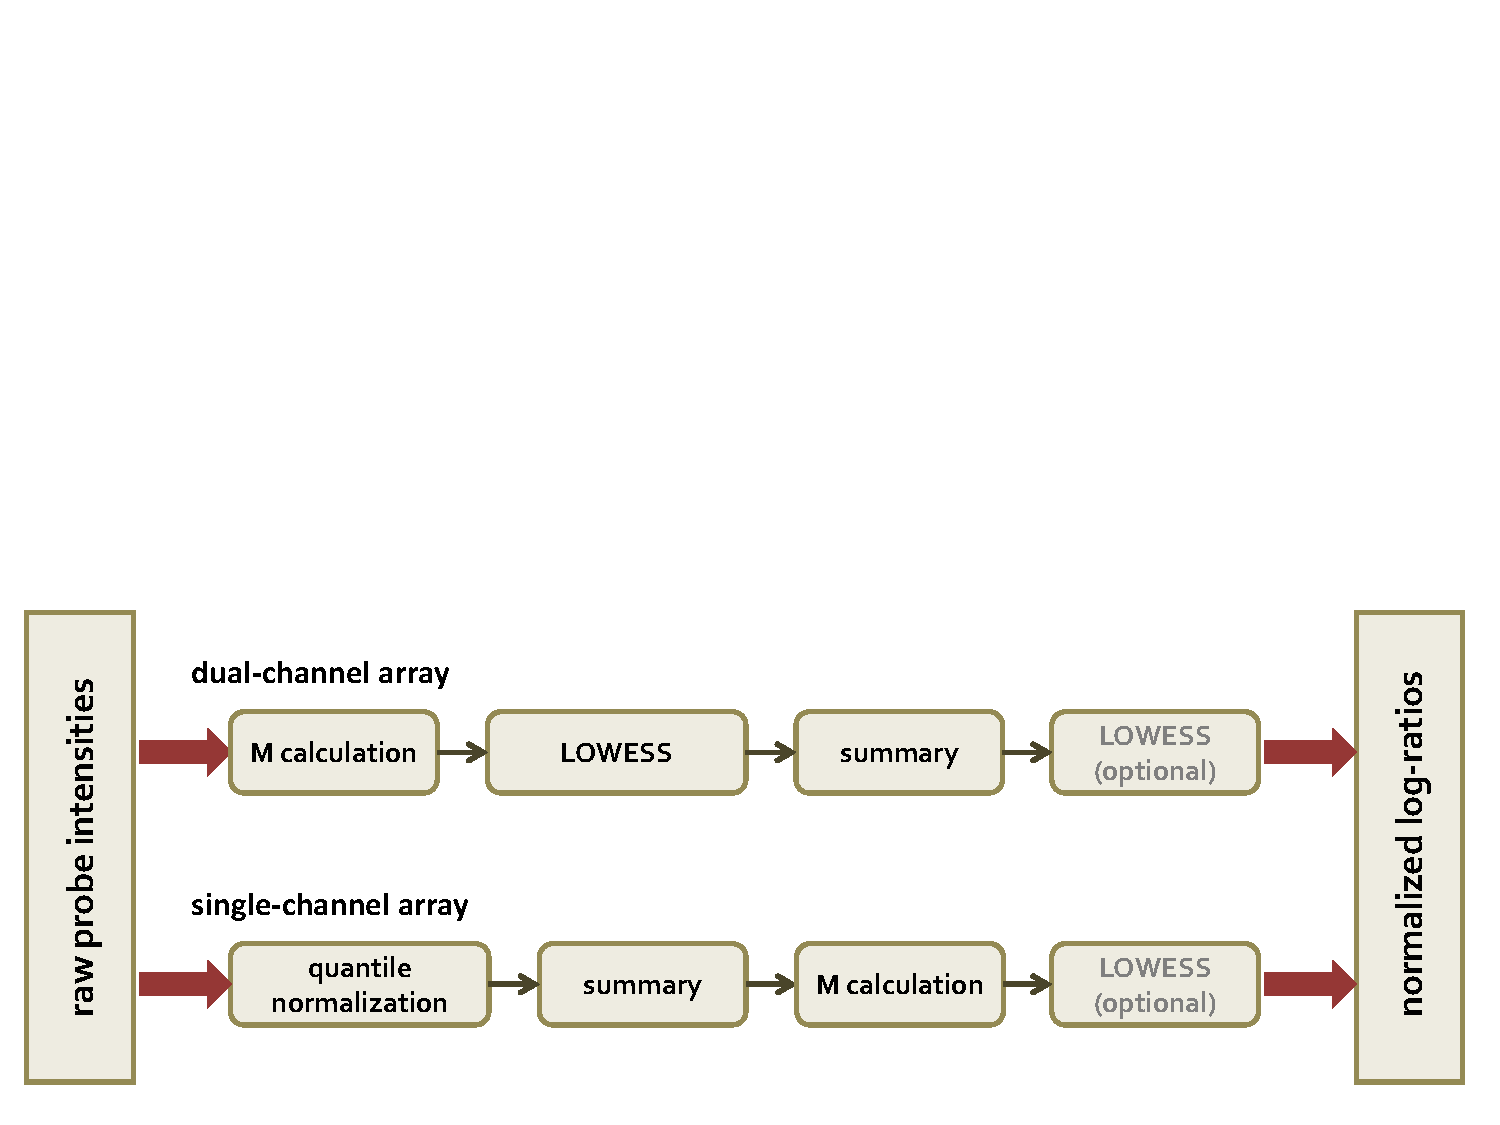
\includegraphics[trim=0cm 0.5cm 0cm 9.5cm, clip=true, width=1\textwidth]{COMMAND_pipelines.pdf}
  \caption[Default pipelines for compendium raw data homogenization]{
    \textbf{Default pipelines for compendium raw data homogenization}}
  \label{fig:command-pipelines}
\end{figure}
%
After log-ratios are calculated for each experiment individually, they are
integrated into one big compendium data matrix containing the data of all the
processed experiments.
%%
%% The final compendium then integrates per-contrast log-ratios
%% across experiments into one data matrix in which there is zero
%% (missing value) or one measurement for each gene in each
%% contrast.

\subparagraph{Multiple-chip platform data normalization}\label{sec:command-multichip-norm}
For a multiple-chip platform, we first followed the same procedure to
normalize data and calculate the log-ratio for each chip separately.
%
Then an additional step is introduced, in which the log-ratios from multiple
chips of the same platform are combined per contrast.
%
Although the chips of a multiple-chip platform are designed to be
complementary, sometimes there are a few genes that are measured on more than
one chip generating multiple expression values per gene.
%
To obtain a single gene expression value per contrast, the median is taken
over the multiple chips to obtain one final value for each gene.
% Take median here as it is more stable against outliers from different arrays


\subsubsection{Data publishing}
%
After internal control, a new compendium are released for public access.
%
An existing compendium can be updated in two fashions, an incremental revision
and a new release.
%
A \textit{revision} adds extra experiments into the current version of the
compendium providing more data.
%
The new data are collected and processed independently, and directly
integrated into the data of the current vesion of compendium after quality
check.
%
Over the time, as the understanding of the genome advances, there can be a
genome revision for a species in which its gene annotations change.
%
Recall that our compendium is a matrix whose rows correspond to genes, the
change of gene annotation will change the number of rows this matrix has.
%
In this case, a \textit{release} is initialized creating a new version of the
compendium incorporating the latest gene annotations.
%
To create a release, the new gene annotations are first imported into the
system, then the platform annotations are updated to this latest gene
annotations, next all experiments available in the current version are
homogenized again utilizing the updated platform annotations to generate the
data matrix for a new version of the compendium, and at last after quality
check, the new version is released for public access.





\subsection{COMMAND web system}


%% - web browser based frontend (user friendly, guidiance) 
%% - ruby based scripts (facilitate development and adaption, automated tasks) 
%% - rigid database design (a balance between size and utility) 

%% apache server + mysql db; javascript, ruby, php, etc 


As utilizing our methodology to create compendium is a complex multiple step
process, a web system named COMMAND (COMpendium MANagement Desktop) has been
develope integrating the methodology with a web interface to facilitate
compendium creation and maintenance.
%
The system is composed of three components, the backend providing core
functionalities for compendium creation, the MySQL database to store the data
collected from online repository and the content of created compendia, and the
web service providing the front-end that interacts with users.  A Apache
server interfaces the communications between those components.
%
The functionalities provided in the backend are computationally intensive and
require no human interaction.  These include but not limited to compendium
initialization, experiment information retrieval, raw data download, automatic
data parsing, data homogenization, and publishing.
%
The peripheral functionalities are implemented directly in the web system,
such as, user control and management, new compendium initialization, etc.  So
are those functionalities require human interactions, such as, various manual
inspection functions, data annotation, etc.  Additionally, data dependencies
between various steps of the metholodogy is controlled through web interface.


% Availability
\paragraph{Availability} 
The whole compendium creation system can be installed and configured to run
on any LAMP server with Matlab runtime environment installed.  Practically,
the system supports a dedicated MySQL server % and a separate computation server
to improve the performance.  The code is not publically avaiable but
can be provided upon requirement.



%% \textbf{Database design} skipped, briefly covered in the compendium schema
%% section
%
%% http://www.codeproject.com/Articles/359654/important-database-designing-rules-which-I-fo
%
%% a modular structure that is the balance between 
%% - normalize to reduce redundancy
%% - de-normalization to improve performance
%% - database views as a middelware (refer below)
%
%% "a dimension and fact design"
%
%% A \textbf{middleware layer} was designed to provide a high-
%% level data model and application program interface to
%% insulate the details of the database schema from user
%% applications. 


%% \textbf{system architecture}

%% The system architecture is modular (a figure). 

%% 5 subsystems: data parsing (interface, integrated data from both
%% repositories), annotation (interface, ??), homogenization, compendium data management
%% (release, revision, etc), system management (user management,
%% compendium management (properties, new compendium, etc) ).

%% brief about extra modules: system namagement, compenidum data management 
%% (release \& revision for data update,  release process)

%% \cite{Petryszak2013} ATLAS2013 p4  'Atlas infrastructure development'





\section{Results and Discussion}

%% Public repositories such as GEO and ArrayExpress provides a centralized
%% storage for expression data, and a set of tools for data submission and
%% retrieval.
%% %
%% By enforcing MIAME guideline, the data quality and reproducibility
%% have been greatly improves.
%% %
%% However, though abundant data are available for a species, the individual
%% experiment still remains isolated and disintegrated due to the pervailed
%% data inconsistencies, inhibiting either globally studying a species in a
%% top-down system biology manner or locally exploring relevant experiments
%% for data comparison or neo-target identification.
%% %

Here, we present a methodology that is capable to integrate high quality
expression data of different experiment and platform origin in a consistent
manner, and creates a species-wise expression compendium accompanied with
high quality manually curated annotations that facilitates both the global
scale analysis and the targeted data exploration.
%
%% \textbf{We created a methodology and created COMMAND system}
Although the abundant data is publically available on repositories such as
GEO and ArrayExpress, the individual experiment still remains isolated and
disintegrated due to the prevailed data inconsistencies, preventing the
utility of an integrated analysis over large number of experiments.
%
Our methodology is specifically designed to tackle this issue by creating a
consistent data set across the experiment and platform boundary that
facilitates efficient data exploration.


Similar efforts that directly integrating publically available data across
experiments do exist, e.g., M$^{\textrm{3D}}$ \cite{Faith2008} and
Genevestigator \cite{Hruz2008}.
%
Centering only on the data generated by single platform (mostly
Affymetrix), these efforts focus mainly on resolving the issue of
inconsistently normalized data and on manual experiment metadata curation.
%
The platform restriction, although simplifies data collection and
normalization tasks, limits the amount of data can be integrated into the
compendium.
% As Affymetrix array reports gene expression intensity, the data in these
% compendia are log-scale absolute intensities.
Our methodolgy does not impose such a limitation, instead tries to
incorporate as much data as possible by integrating data across different
platforms.

To achieve our goal, we faces two extra challenges, the data collection and
the data normalization and integration.
%
When compared to that of the single-platform compendium, the data
collection is more complicated in two aspects.
%
First, there lacks of standard formats to report the raw expression values
measured on various platforms.  Especially for dual-channel platforms that
probe expression values for two biological samples at a time, it is not
simple to identify and extract the desirable data for each channel from
data table of variant formats.
%
Second, as two samples are hybridized on an array, the corresponding sample
of the data generated in each channel must be correctly identified to
guarantee that the proper experimental metadata information is used for
annotation that is crutial for downstream data analysis and result
interpretation.
%
To this end, a semi-automatic raw data parsing subsystem capable of
handling data format heterogeneity and extrapolating correct data sample
associations is developed.
%
In a majority of cases, experiment data available online are handled
automatically by the system, avoiding time-consuming human intervention.
%
When necessary, it do can incorportate extra information obtained from
manual data inspection to extract data.
%
The system enables us to process a large number of heterogeneous data
efficiently.


To handle the data generated from different types of platforms also
complicates the data normalization and integration.
%
In our system, platform specific normalization schema is utilized to handle
particular issues associated with each type of platform, for example, LOWESS
to correct dye bias in dual-channel arrays, quantile normalization to reduce
the variance among replicates for single-channel platform.
%
Different types of platform produce different expression measurements.
Single-channel platform generates absolute intensity value for each gene.
Whereas, for dual-channel platform, log-ratio is generally preferred as
caclulated between the intensities obtained from the same sport, it
effectively removes undeirable spot and array effects from the data.
%
The log-ratio has been shown to improve consistency among results obtained
across differeny microarray types \cite{Shi2006}, hence it is adopted as
the type of the expression data for our compendium.
%
To calculate log-ratio for all data, the concept of contrast is introduced,
in which one sample designated as the test is compared with the other
sample as the reference to reveal differentially expressed genes.
%
For a dual-channel array, a contrast is naturally defined between samples
hybridized to it.
%
For an experiment using single-channel array, one or more refernece samples
are manually chosen based on the platform used and the nature of the
experiment.
%
The log-ratio can then be effectively calculated for each contrast with a
clear biological meaning representing the observed gene expression
changes induced by either the external perturbation(s) or the internal
differences between samples.
%
Furthermore, for experiments using single-channel platform, it has been shown
that the log-ratios calculated between samples from the same batch (experiment
and platform) effectively removes undesirable batch-effects \cite{Luo2010}.


The gene expression data are useful only when the accompany sample information
is available.  We have also taken great care to provide an extensive formal
contrast annotation and associated that with higher level condition ontology.
%
As our compendium data are the log-ratios representing gene expression
changes, our annotation focuses on specifying the differences between the pair
of samples of a contrast.
%
This is different from that of the single-platform compendium aiming to
specify the complete information of each sample.


The methodology described here enables us to create a cross-platform
expression compendium.
%
Through integrating the data across different platforms, the methodology has
two advantages compared to the existing single-platform one.  First, it
enables the creation of the compendium that incorporate much more data.
Second, it enables to create a sizable compendium for species which there is
no dominat platform exists.
%
Utilizing this methodology, we successfully created three bacterial
compendia for {\it Escherichia coli}, {\it Bacillus subtilis}, and {\it
  Salmonella enterica serovar Typhimurium}.  The \textit{E. coli} one is
the largest currently available, and the last two are unique.
%
The details of these bacterial compendia are described in chapter
\ref{ch:colombos}.
%
Furthermore, the methodology has been adapted to construct compendium for
Eukaryotes.
%
A proof-of-concept compendium for \textit{Zea mays} (chapter \ref{ch:magic})
has been created, providing high data consistency by incorportaing a complete
reannotation of the existing platforms based on the lastest genome release and
the extended annotations reflecting the complex structure and life style of a
plant.



%% ArrayExpress a lot of changes in SDRF file and the raw datas without
%% notifications, hard for developer to track and code needs to be adapted,
%% although the information provided are now more consistent ...


%% \textbf{Choice of extracting raw intensity data, especially problematic for dual-channel arrays}

%% Although widely accepted community guideline such as MIAME \cite{Brazma2001}
%% greatly improved the reproducibility of experiments and the understanding of
%% the data by promoting a more precise description of experimental procedure, it
%% fails to provide detailed guidelines that facilitate the computerized analysis
%% of the data due to the lack of specifications for rigid data reporting formats.

%% \textbf{Choice of contrast and log-ratio}

%% \textbf{Check Introduction - Log-ratios and condition contrasts by 
%% \textit{kristof}}

%% In case a multiple-chip platform is used, a direct data merge across
%% chips is possible only for log-ratios data instead of intensity data,
%% as log-ratio cancel out the batch effects, whereas the batch effects
%% contained in the intensity data cannot be readily removed because
%% little or none genes are in common across chips.

%% \textbf{Choice for data homogenization}

%% handling different platforms, different strategies, compare with M3D and
%% genevestigator compendium








%%%%%%%%%%%%%%%%%%%%%%%%%%%%%%%%%%%%%%%%%%%%%%%%%%
% Keep the following \cleardoublepage at the end of this file, 
% otherwise \includeonly includes empty pages.
\cleardoublepage


% vim: tw=70 nocindent expandtab foldmethod=marker foldmarker={{{}{,}{}}}
